\documentclass{article}


% if you need to pass options to natbib, use, e.g.:
% \PassOptionsToPackage{numbers, compress}{natbib}
% before loading neurips_2025


% ready for submission
\usepackage{neurips_2025}
% to compile a preprint version, e.g., for submission to arXiv, add add the
% [preprint] option:
%     \usepackage[preprint]{neurips_2025}


% to compile a camera-ready version, add the [final] option, e.g.:
%     \usepackage[final]{neurips_2025}


% to avoid loading the natbib package, add option nonatbib:
%    \usepackage[nonatbib]{neurips_2025}


\usepackage[utf8]{inputenc} % allow utf-8 input
\usepackage[T1]{fontenc}    % use 8-bit T1 fonts
\usepackage{hyperref}       % hyperlinks
\usepackage{url}            % simple URL typesetting
\usepackage{booktabs}       % professional-quality tables
\usepackage{amsfonts}       % blackboard math symbols
\usepackage{nicefrac}       % compact symbols for 1/2, etc.
\usepackage{microtype}      % microtypography
\usepackage{xcolor}         % colors
\usepackage{graphicx}
\usepackage{multirow}
\usepackage{multicol}
\usepackage{adjustbox}
\usepackage{makecell}
\usepackage{arydshln,subcaption,xcolor}
\usepackage{graphicx}
\usepackage{multirow}
\usepackage{titlesec}
\usepackage{caption}
% \usepackage{fontspec}
\usepackage{colortbl}
\usepackage[margin=1in]{geometry}
% \setmainfont{Times New Roman}
\usepackage{wrapfig}
\usepackage{lipsum}






\title{RESPIN-S1.0 Corpus: A read speech corpus of 10000+ hours in dialects of nine Indian Languages}

\author{%
}

\begin{document}
\maketitle
% \tableofcontents

\begin{abstract}
We introduce \textbf{RESPIN-S1.0}, the largest publicly available dialect-rich read speech corpus for Indian languages, comprising over 10,000 hours of validated audio spanning nine major languages -- Bengali, Bhojpuri, Chhattisgarhi, Hindi, Kannada, Magahi, Maithili, Marathi, and Telugu. Indian languages are characterized by high dialectal variation and are spoken by populations that are often digitally underserved. Existing speech corpora typically represent only standard dialects and lack domain relevance. RESPIN-S1.0 fills this critical gap by collecting speech across 38+ dialects and two high-impact domains: agriculture and finance. Text data was carefully composed by native dialect speakers and validated via a robust pipeline involving both automatic and manual checks. Over 200,000 utterances were recorded through a crowdsourced mobile application by native speakers and subsequently categorized into clean, semi-noisy, and noisy slabs based on transcription quality. The clean slab alone exceeds 10,000 hours. RESPIN also provides speaker metadata, phonetic lexicons, and dialect-aware train-dev-test splits to ensure reproducibility. To benchmark performance, we evaluate a range of ASR models -- TDNN-HMM, E-Branchformer, Whisper, IndicWav2Vec2, and SPRING SSL models -- and find that fine-tuning on RESPIN significantly improves recognition accuracy over existing pretrained models. A subset of RESPIN-S1.0 has already supported community efforts through challenges such as the SLT Code Hackathon 2022 and MADASR@ASRU 2023/2025, with over 1200 hours of data released publicly. This resource supports research in dialectal ASR, LID, DID, and speech-related areas, and sets a new standard for inclusive, dialect-rich corpora in multilingual, low-resource settings.
\end{abstract}

% %%%%%%%%%%%%%%%%%%%%%%%%%%%%%%%%%%%%%%%%%%%%%%%%%%%%%%%%%%%%%%%%%%%%%%%%

\section{Introduction}

India's vast linguistic diversity -- with 22 scheduled languages and hundreds of dialects~\footnote{\url{https://censusindia.gov.in/nada/index.php/catalog/42561/download/46187/Language_Atlas_2011.pdf}} -- necessitates speech technologies that support local languages to ensure inclusivity. However, development in this space remains limited due to the scarcity of curated audio-text datasets~\cite{10.1007/978-3-030-95711-7_8}, especially for dialectal variation~\cite{gumperz1961speech}. Roughly 64\% of India’s population lives in rural areas, and 57.8\% belong to agricultural households~\cite{wb}, yet ASR research has largely focused on English or standard language forms~\cite{hari_thesis}. Existing corpora often cover only standard dialects~\cite{gumperz1961speech,Mandal1990}, leading to poor performance on regionally diverse speech.

To address this, RESPIN-S1.0 introduces a large-scale, multi-dialectal, multi-domain read speech corpus for nine Indian languages -- Bengali, Bhojpuri, Chhattisgarhi, Hindi, Kannada, Magahi, Maithili, Marathi, and Telugu. Languages were selected based on speaker population, socio-economic indicators, and availability of resources. Figure~\ref{fig:dialect_distribution_india_map} shows the district-level language distribution and dialect breakdown. RESPIN is the first public corpus to provide large-scale dialectal data for Bhojpuri, Chhattisgarhi, and Magahi. The pipeline -- from sentence composition to audio validation -- was conducted at the dialect level to preserve linguistic integrity. It also includes manually verified phonetic lexicons (as per ILSL guidelines~\cite{Samudravijaya2021}) and rich speaker metadata (e.g., pincode, gender, age group).

\begin{figure}
    \centering
    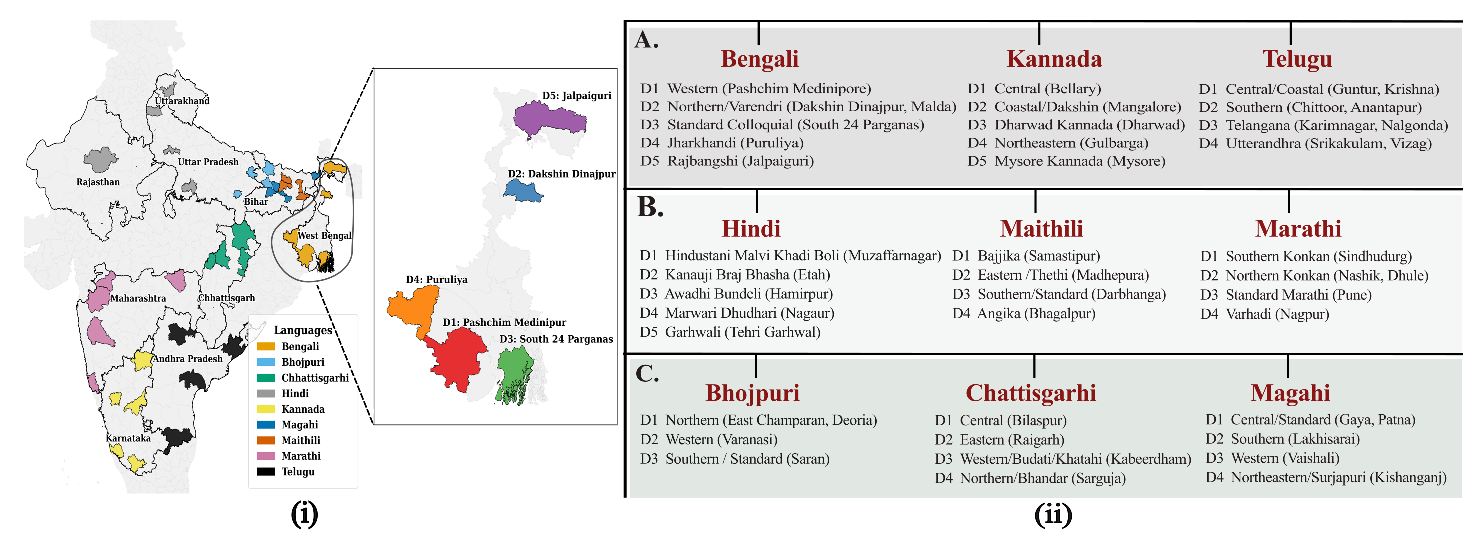
\includegraphics[width=0.99\linewidth]{Styles/figures/figure-1-neurips-v2_mod.eps}
    \caption{(i) District-level distribution of the nine RESPIN languages across India, based on the 2011 Census (illustrative, not to scale). Each language is shown in a distinct color. A sample inset shows dialect-wise representation for Bengali. (ii) Language classification: A -- Scheduled, non-Devanagari; B -- Scheduled, Devanagari; C -- Non-scheduled, Devanagari.}
    \label{fig:dialect_distribution_india_map}
    \vspace{-10pt}
\end{figure}

To promote reproducibility, RESPIN provides train/dev/test splits, dialect-level metadata, and ASR benchmarks using TDNN-HMM~\cite{povey18_interspeech}, E-Branchformer~\cite{Kwangyoun_EBF_SLT2022}, Whisper~\cite{Radford_whisper2023}, and SSL models like IndicWav2Vec2~\cite{javed2021building} and SPRING-Data2Vec~\footnote{\url{https://asr.iitm.ac.in/models}}. Fine-tuning on RESPIN consistently improves ASR performance over models trained on external corpora. RESPIN has already enabled multilingual ASR research through the SLT Code Hackathon 2022~\footnote{\url{https://sites.google.com/view/slt-team}} and MADASR challenges (ASRU 2023, ASRU 2025)~\footnote{\url{https://sites.google.com/view/respinasrchallenge2025/home}}, where 1200+ hours were released to the participants. By capturing India’s linguistic depth, RESPIN advances inclusive voice technologies for underserved communities in the Global South.\vspace{-3mm}


% \section{Introduction}

% Speech is the most natural and accessible mode of human communication. According to the \emph{Census of India 2011}, India is home to 22 scheduled languages and hundreds of dialects. This immense linguistic diversity highlights the need for speech technologies that support local languages and dialects to ensure inclusivity and accessibility across all sections of the population.

% Despite increasing demand, the development of speech-based technologies in India remains constrained by the limited availability of curated audio and text data \cite{10.1007/978-3-030-95711-7_8}. This challenge is further amplified by the presence of numerous dialects within each language, which often differ significantly in phonetics, vocabulary, and syntax \cite{gumperz1961speech}.

% As per World Bank staff estimates based on the United Nations Population Division's World Urbanization Prospects, approximately 64\% of India’s population resides in rural areas, with nearly 57.8\% belonging to agricultural households \cite{wb}. A majority of these individuals are non-English speakers, yet speech recognition research has historically focused on English or standard language varieties \cite{hari_thesis}. To build inclusive voice technologies for rural, low-literacy populations, large-scale data collection covering multiple dialects is essential.

% Existing Indian speech corpora typically represent only the standard dialects of languages, targeting formal or educated speech \cite{gumperz1961speech,Mandal1990}. This results in under-representation of regional speech diversity in modern ASR systems. RESPIN-S1.0 addresses this gap by systematically identifying, collecting, and democratizing access to dialect-rich speech and language data. The initiative aims to empower India’s tech ecosystem to build accurate and affordable speech and NLP solutions, particularly for high-impact domains such as banking and agriculture.

% RESPIN-S1.0 is a large-scale, multi-dialectal, multi-domain Indian read speech corpus focused on two economically critical sectors: agriculture and finance. As shown in Figure~\ref{fig:dialect_distribution_india_map}, RESPIN-S1.0 spans nine Indian languages and their dialects -- Bengali, Bhojpuri, Chhattisgarhi, Hindi, Kannada, Magahi, Maithili, Marathi, and Telugu. These languages were selected based on multiple criteria, including speaker population size, poor state-level socio-economic indicators, limited existing speech technology resources, and their potential for high-impact societal use cases. %\footnote{Selection rationale based on internal analysis and Census 2011 statistics.} [You can optionally cite sources like NITI Aayog reports, poverty index, or rural demographics.]

% To the best of our knowledge, RESPIN-S1.0 is the first publicly available, large-scale speech corpus for dialects of Bhojpuri, Chhattisgarhi, and Magahi -- three low-resource Indian languages. The entire data creation pipeline -- from text composition and validation to audio recording and validation -- was executed at the dialectal level to maintain dialectal integrity. RESPIN is the largest such initiative in India where dialect-informed text composition was central to data design. The corpus also includes manually verified phonetic lexicons aligned with ILSL guidelines and comprehensive speaker metadata, including pincode, age group, and gender.

% \begin{figure}
%     \centering
%     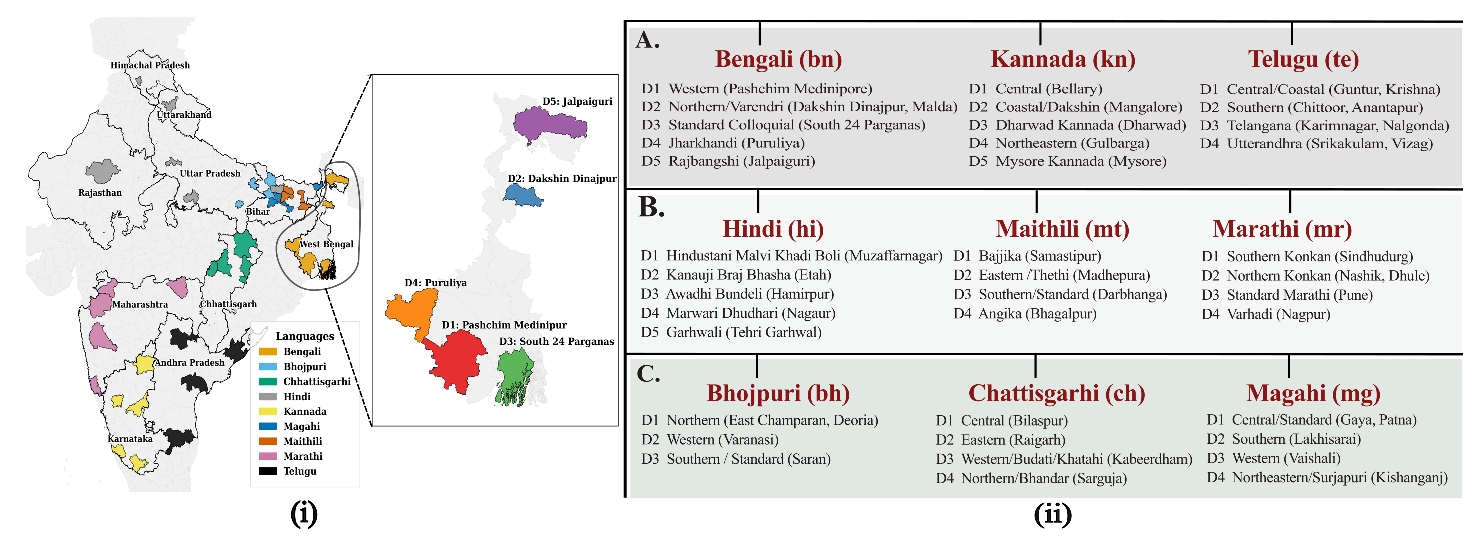
\includegraphics[width=0.99\linewidth]{Styles/figures/figure-1-neurips-v2.eps}
%     \caption{(i) District-level distribution of the nine RESPIN languages across India, based on the 2011 Census (illustrative, not to scale). Each language is shown in a distinct color. A sample inset shows dialect-wise representation for Bengali. (ii) Language classification: A -- Scheduled, non-Devanagari; B -- Scheduled, Devanagari; C -- Non-scheduled, Devanagari.}
%     \label{fig:dialect_distribution_india_map}
%     \vspace{-10pt}
% \end{figure}

% To promote reproducibility and standardization in research, RESPIN-S1.0 provides predefined train/dev/test splits, dialect-level metadata, and benchmark results from several ASR systems including TDNN-HMM, E-Branchformer, Whisper, and self-supervised learning models such as IndicWav2Vec2 and SPRING-Data2Vec. Fine-tuning these models on RESPIN significantly improves ASR performance compared to training solely on publicly available corpora.

% RESPIN-S1.0 has already had real-world impact through its use in the SLT Code Hackathon and the MADASR challenge series (ASRU 2023, ASRU 2025), where 1200+ hours of RESPIN data were released for multilingual, multi-dialectal ASR research. By capturing India's linguistic diversity and enabling inclusive voice technologies, RESPIN-S1.0 lays the foundation for a new generation of speech systems tailored to underserved communities in the Global South.


% The key contributions of RESPIN-S1.0 ASR database are as follows \textcolor{red}{TODO}:
% \begin{enumerate}
    % \item Large-scale read speech corpus for 9 Indian languages with dialectal varieties covering two domains: agriculture and finance.
    % \item First ever publicly available speech corpora for low-resource languages: Chhattisgarhi and Bhojpuri.
    % \item Apart from Hindi, which is already amply available, we open-source at least twice the volume of speech data currently available for each of these languages.
    % \item Dialectal integrity is maintained at each step of the data creation process, starting from text composition, text validation, audio recording, and audio validation, etc.
    % \item first largest initiative for Indian languages where text data was composed and validated at the dialectal level
    % \item Human-validated phonetic lexicons following ILSL guidelines.
    % \item Comprehensive speaker and location metadata (including pin codes), age group
    % spkr info (pincode, age, gender)&. 
% \end{enumerate}


% \section{Literature Survey}
%  \label{sec2}

 % \begin{table*}[!ht]
% % \centering
% % \caption{}
% % % \vspace{-0.3cm}
% % \label{tab:lang}
% % \resizebox{\textwidth}{!}{
% % \begin{tabular}{|l|l|l|l|l|}
% % \hline
% % \textbf{Dataset} &
% %   \textbf{\begin{tabular}[c]{@{}l@{}}Number of\\  languages\end{tabular}} &
% %   \textbf{\begin{tabular}[c]{@{}l@{}}Number of\\  hours\end{tabular}} &
% %   \textbf{Domain / Source} &
% %   \textbf{\begin{tabular}[c]{@{}l@{}}Dialectal \\ Information\end{tabular}} \\ \hline
% % Low Resource ASR Challenge IS 2018 &
% %   3 &
% %   150 &
% %   NA &
% %   NA \\ \hline
% % IIIT-H Indic &
% %   7 &
% %   12.84 &
% %   Wikipedia &
% %   NA \\ \hline
% % Open-source Multi-speaker Speech Corpora &
% %   6 &
% %   38.09 &
% %   NA &
% %   NA \\ \hline
% % Step-by-Step Process for Building TTS Voices &
% %   1 &
% %   2.93 &
% %   NA &
% %   NA \\ \hline
% % Resources for Indian languages &
% %   13 &
% %   389.6 &
% %   \begin{tabular}[c]{@{}l@{}}children stories, literature, \\ science, tourism, newspapers, \\ websites, blogs\end{tabular} &
% %    \\ \hline
% % IIITH-ILSC &
% %   22 &
% %   103.5 &
% %   NA &
% %   NA \\ \hline
% % Common Voice &
% %   1 &
% %   5 &
% %   Wikipedia &
% %   NA \\ \hline
% % \begin{tabular}[c]{@{}l@{}}Multilingual Speech Corpus in Low‑Resource \\ Eastern and Northeastern Indian Languages for \\ Speaker and Language Identification\end{tabular} &
% %   4 &
% %   19.75 &
% %   NA &
% %   \begin{tabular}[c]{@{}l@{}}dialect variations but \\ no proper labels\end{tabular} \\ \hline
% % NISP &
% %   5 &
% %   24.83 &
% %   news articles &
% %   \begin{tabular}[c]{@{}l@{}}Regional information \\ of speaker is given\end{tabular} \\ \hline
% % \begin{tabular}[c]{@{}l@{}}Automatic Speech Recognition in Sanskrit: \\ A New Speech Corpus and Modelling Insights\end{tabular} &
% %   1 &
% %   78 &
% %   prose, poems &
% %   NA \\ \hline
% % Shrutilipi &
% %   12 &
% %   6440 &
% %   news archives from All India Radio &
% %   NA \\ \hline
% % \begin{tabular}[c]{@{}l@{}}Multilingual and code-switching ASR challenges for\\ low resource Indian languages\end{tabular} &
% %   6 &
% %   600 &
% %   \begin{tabular}[c]{@{}l@{}}Agriculture, Finance and Healthcare \\ and storybooks.\end{tabular} &
% %   YES \\ \hline
% % IndicVoices-R &
% %   22 &
% %   1704 &
% %   NA &
% %   NA \\ \hline
% % IndicVoices &
% %   13 &
% %   7348 &
% %   \begin{tabular}[c]{@{}l@{}}legal, governance, history, geography,\\ tourism, stem, religion, business, sports, \\ entertainment, health, culture and news etc\end{tabular} &
% %   145 Indian districts \\ \hline
% % \begin{tabular}[c]{@{}l@{}}Using cross-model learnings for the Gram Vaani \\ ASR Challenge 2022\end{tabular} &
% %   1 &
% %   1100 &
% %   NA &
% %   \begin{tabular}[c]{@{}l@{}}regional/dialectal \\ variations but no labels\end{tabular} \\ \hline
% % \begin{tabular}[c]{@{}l@{}}Subword Dictionary Learning and Segmentation\\ Techniques for Automatic Speech Recognition in Tamil\\ and Kannada\end{tabular} &
% %   2 &
% %   497 &
% %   NA &
% %   NA \\ \hline
% % \begin{tabular}[c]{@{}l@{}}Crowdsourcing Speech Data for Low-Resource Languages \\ from Low-Income Workers\end{tabular} &
% %   1 &
% %   109 &
% %   \begin{tabular}[c]{@{}l@{}}elements of linguistic pride, \\ the centrality of the communal\\ aspect of the work, \\ and the importance of storytelling and\\ commensurate lack of previously available \\ reading material.\end{tabular} &
% %   NA \\ \hline
% % Svarah &
% %   1 &
% %   9.6 &
% %   \begin{tabular}[c]{@{}l@{}}painting, cooking, gardening, knitting and \\ stitching, travelling,\end{tabular} &
% %   65 Indian regions \\ \hline
% % SPRING-INX &
% %   10 &
% %   2000 &
% %   \begin{tabular}[c]{@{}l@{}}weather, different types of\\ news, entertainment, health, \\ agriculture, education,  jobs, \\ BPO (Business Process Outsourcing) etc.\end{tabular} &
% %   4 dialects per language \\ \hline
% % SPIRE-SIES &
% %   1 &
% %   170 &
% %   NA &
% %   NA \\ \hline
% % GramVaani &
% %   1 &
% %   1108 &
% %   \begin{tabular}[c]{@{}l@{}}hyperlocal news reported by citizen journalists, \\ questions on agriculture or \\ health, grievances related to access to social \\ entitlements, and also folk songs and poems\end{tabular} &
% %   hindi from 25 districts \\ \hline
%  \end{tabular}}
% \end{table*}

\section{Background}
Dialectal datasets are vital for building accurate and inclusive speech technologies, as they reflect real-world language use, improve recognition performance across regions, ensure access for marginalized communities, support critical public service applications, and help preserve linguistic diversity. %Despite progress in speech processing, most world languages and dialects remain underrepresented due to limited datasets. 
Continued investment in community-driven, open-access, and dialect-rich data collection is essential for building equitable and effective speech technologies. As mentioned in \cite{yvideo}, treating dialects respectfully is crucial in supporting the most marginalized. 

Across the world, several initiatives have emerged to create dialect-rich speech datasets to support inclusive speech technologies. In the Arabic-speaking world, CASABLANCA \cite{talafha-etal-2024-casablanca} and MADAR \cite{bouamor-etal-2018-madar} provide large-scale, multi-dialect corpora to capture the diversity of regional Arabic. In China, efforts like AISHELL \cite{bu2017aishell1opensourcemandarinspeech} and THCHS-30 \cite{THCHS30_2015} focus on Mandarin but lay foundational work for dialectal speech research. In Africa, Masakhane ASR \cite{azime2023masakhaneafrisentisemeval2023task12} and CMU Wilderness \cite{8683536} aim to fill the gap for underrepresented African languages and dialects through open, community-led efforts. Together, these initiatives represent significant strides toward bridging the global speech technology divide.

% \begin{table}[!ht]
% \caption{Existing Indic Datasets}
% % \centering
% % \vspace{-0.3cm}
% \label{tab:datasets}
% \resizebox{0.9\textwidth}{!}{
% \begin{tabular}{l|l|l|l|l|l|l|l}
% \hline
% \textbf{Dataset} & \textbf{Languages} & \textbf{Domains} & \textbf{Districts} & \textbf{Hours} & \textbf{Speakers} & \textbf{Sentences}& \textbf{Source}\\
% \hline
% INDICVOICES~\cite{javed2024indicvoices} & 13 & 52 & 145 & 7348 & 16237 & 11,00,000+ & Wikipedia, Composed, Spontaneous\\
% % \vspace{0.15cm}
% INDICVOICES-R~\cite{sankar2024indicvoices} & 22 & multi & multi & 1704 & 10496 & NA & NA \\
% % \vspace{0.1cm}
% Kathbath~\cite{javed2023indicsuperb} & 12 & multi & 203 & 1684 & 1217 & 12,00,000+ & IndicCorp (Web data) \\
% Shrutilipi~\cite{bhogale2023effectiveness} & 12 & multi & NA & 6457 & NA & 33,00,000 & All India Radio \\
% NPTEL~\cite{bhogale2023vistaar} & 8 & 1 & NA & 857 & NA & NA & Lectures \\
% Svarah~\cite{javed2023svarah} & 1 & 9 & 65 & 9.6 & 117 & NA & Wikipedia, Prompts, Spontaneous \\
% SPRING-INX~\cite{gangwar2023spring} & 10 & mutli & 40+ & 2000 & 7609 & NA & NA \\
% SPIRE-SIES~\cite{singh2023spire} & 1 & NA & NA & 193 & 1607 & NA & NA \\
% FLEURS~\cite{conneau2023fleurs} & 13 & NA & NA & 156 & 39 & NA & Wikipedia \\
% Gram Vaani~\cite{bhanushali2022gram} & 1 & multi & 25 & 1108 & NA & NA & Spontaneous Speech \\
% IISc-MILE~\cite{diwan2021multilingual} & 2 & NA & NA & 497 & 1446 & NA & NA \\
% MUCS~\cite{diwan2021multilingual} & 3 & 4 & 4 (for Odia) & NA & 310 & 9080 & NA\\
% Vāksañcayah~\cite{adiga2021automatic} & 1 & 8 & NA & 78 & 27 & 46,000 & Online stories \\
% E\&NE languages~\cite{basu2021multilingual} & 4 & NA & multi & 19.75 & NA & NA & NA \\
% NISP~\cite{kalluri2021nisp} & 6 & NA & NA & 56.86 & 345 & NA & news, TIMIT \\
% CommonVoice~\cite{commonvoice:2020} & 8? & 4? & NA & 373? & NA & NA & Wikipedia, Composed \\
% CMS~\cite{he2020open} & 6 & NA & NA & 35 & 243 & NA & Composed \\
% IITB-MSC~\cite{abraham2020crowdsourcing} & 1 & 1 & 1 & 109 & 36 & 3000 & Textbooks \\
% IndicSpeech~\cite{srivastava2020indicspeech} & 3 & NA & NA & 24 & 3 & 42,046 & Online news \\
% MSR Challenge~\cite{srivastava2018interspeech} & 3 & NA & NA & 150 & 1286 & 1,02,397 & NA \\
% Google TTS~\cite{sodimana2018step} & 1 & NA & NA & 3 & 6 & NA & NA\\
% IIITH-ILSC~\cite{vuddagiri2018iiith} & 23 & NA & NA & 103.5 & 1150 & NA & NA \\
% IndicTTS~\cite{wilkinson2016open} & 13 & 4+ & NA & 389.6 & 26 & NA & Literature, newspapers \\
% IIITH-ISD~\cite{prahallad2012iiit} & 7 & NA & NA & 11 & 35 & 1000 & Wikipedia \\
% \hline
% \vspace{-0.25 cm}
% & & & & & &\\
% \textbf{RESPIN-S1.0} & \textbf{9} & \textbf{2} & \textbf{38+} & \textbf{10,416.58} & \textbf{18,000+} & \textbf{2,09,822} & \textbf{Composed}\\
% \hline
% \small{NA $-$ Complete Information Not Available}
% \end{tabular}\vspace{-10mm}

% }
% \end{table}

\begin{table}[!ht]
\vspace{-5mm}
\centering
\caption{Existing Indic Datasets}
\label{tab:datasets}
\resizebox{0.9\textwidth}{!}{
\begin{tabular}{l l l l r r r l}
\toprule
\textbf{Dataset} & \textbf{Languages} & \textbf{Domains} & \textbf{Districts} & \textbf{Hours} & \textbf{Speakers} & \textbf{Sentences} & \textbf{Source} \\
\midrule
INDICVOICES~\cite{javed2024indicvoices} & 13 & 52 & 145 & 7348 & 16237 & 11,00,000+ & Wikipedia, Composed, Spontaneous \\
INDICVOICES-R~\cite{sankar2024indicvoices} & 22 & multi & multi & 1704 & 10496 & NA & NA \\
Kathbath~\cite{javed2023indicsuperb} & 12 & multi & 203 & 1684 & 1217 & 12,00,000+ & IndicCorp (Web data) \\
Shrutilipi~\cite{bhogale2023effectiveness} & 12 & multi & NA & 6457 & NA & 33,00,000 & All India Radio \\
NPTEL~\cite{bhogale2023vistaar} & 8 & 1 & NA & 857 & NA & NA & Lectures \\
Svarah~\cite{javed2023svarah} & 1 & 9 & 65 & 9.6 & 117 & NA & Wikipedia, Prompts, Spontaneous \\
SPRING-INX~\cite{gangwar2023spring} & 10 & multi & 40+ & 2000 & 7609 & NA & NA \\
SPIRE-SIES~\cite{singh2023spire} & 1 & NA & NA & 193 & 1607 & NA & NA \\
FLEURS~\cite{conneau2023fleurs} & 13 & NA & NA & 156 & 39 & NA & Wikipedia \\
Gram Vaani~\cite{bhanushali2022gram} & 1 & multi & 25 & 1108 & NA & NA & Spontaneous Speech \\
IISc-MILE~\cite{diwan2021multilingual} & 2 & NA & NA & 497 & 1446 & NA & NA \\
MUCS~\cite{diwan2021multilingual} & 3 & 4 & 4 (for Odia) & NA & 310 & 9080 & NA \\
\textnormal{V\=aks\~anca\-yah}~\cite{adiga2021automatic} & 1 & 8 & NA & 78 & 27 & 46,000 & Online stories \\
E\&NE languages~\cite{basu2021multilingual} & 4 & NA & multi & 19.75 & NA & NA & NA \\
NISP~\cite{kalluri2021nisp} & 6 & NA & NA & 56.86 & 345 & NA & news, TIMIT \\
CommonVoice~\cite{commonvoice:2020} & 8? & 4? & NA & 373? & NA & NA & Wikipedia, Composed \\
CMS~\cite{he2020open} & 6 & NA & NA & 35 & 243 & NA & Composed \\
IITB-MSC~\cite{abraham2020crowdsourcing} & 1 & 1 & 1 & 109 & 36 & 3000 & Textbooks \\
IndicSpeech~\cite{srivastava2020indicspeech} & 3 & NA & NA & 24 & 3 & 42,046 & Online news \\
MSR Challenge~\cite{srivastava2018interspeech} & 3 & NA & NA & 150 & 1286 & 1,02,397 & NA \\
Google TTS~\cite{sodimana2018step} & 1 & NA & NA & 3 & 6 & NA & NA \\
IIITH-ILSC~\cite{vuddagiri2018iiith} & 23 & NA & NA & 103.5 & 1150 & NA & NA \\
IndicTTS~\cite{wilkinson2016open} & 13 & 4+ & NA & 389.6 & 26 & NA & Literature, newspapers \\
IIITH-ISD~\cite{prahallad2012iiit} & 7 & NA & NA & 11 & 35 & 1000 & Wikipedia \\
\midrule
\textbf{RESPIN-S1.0} & \textbf{9} & \textbf{2} & \textbf{38+} & \textbf{10,416.58} & \textbf{18,000+} & \textbf{2,09,822} & \textbf{Composed} \\
\bottomrule
\multicolumn{8}{l}{\small \textit{NA} = Information Not Available}
\end{tabular}
}
\end{table}


Table~\ref{tab:datasets} compares major open-source Indic speech corpora across languages, domains, districts, duration, speaker count, and data sources. While many datasets offer broad language coverage and large volumes of audio, they often lack dialectal diversity and regional specificity -- critical for building inclusive ASR systems for rural populations. Most rely on publicly available web content (e.g., Wikipedia, books, news), resulting in generic domain coverage and limited alignment with real-world use. RESPIN-S1.0 addresses these limitations by focusing on agriculture and banking -- domains essential to India’s low-literacy and rural communities -- and by manually composing 2,09,822 sentences to reflect regionally grounded, colloquial speech. Unlike large-scale efforts like INDICVOICES~\cite{javed2024indicvoices} and INDICVOICES-R~\cite{sankar2024indicvoices}, which cover scheduled languages, RESPIN also includes low-resource, non-scheduled languages such as Bhojpuri, Chhattisgarhi, and Magahi, often mislabeled as Hindi dialects. With over 10,000 hours of validated audio from 18,000+ speakers across 38+ dialect-rich districts, RESPIN offers the most comprehensive dialect-aware resource for speech technology in Indian languages. RESPIN aims to empower rural populations by enabling voice-based digital services in their native dialects, fostering trust in speech interfaces, and driving inclusive access for the next 500 million users in India.\vspace{-3mm}


\section{Data collection and Validation pipeline}

\begin{wrapfigure}{r}{0.40\textwidth}
    \centering
    \vspace{-10pt}
    \includegraphics[width=0.4\textwidth]{figures/data_pipeline.png}
    \caption{Data creation pipeline maintaining dialectal integrity.}
    \label{fig:datapipeline}
    \vspace{-10pt}
\end{wrapfigure}

RESPIN is the first large-scale Indian speech corpus to preserve dialectal integrity throughout the data creation process. As shown in Figure~\ref{fig:datapipeline}, the pipeline includes language and dialect selection, manual text composition, multi-stage validation, and speaker-level audio collection. Unlike corpora built from scraped or generic online content, RESPIN focuses on agriculture and finance, with all text and audio created and validated at the dialect level. RESPIN has ensured that all the contributors are valued and supported throughout each stage of development. They remain well-informed and actively engaged with the project's goals, progress, and strategic direction.


% RESPIN is the first large-scale Indian speech corpus to maintain dialectal integrity throughout the data creation process. As shown in Figure~\ref{fig:datapipeline}, the pipeline covers language and dialect selection, manual text composition, multi-stage validation, and speaker-level audio collection and validation. Unlike corpora built from web scraping or generic online content, RESPIN focuses on agriculture and finance, with all text and audio carefully created and validated at the dialect level.


% RESPIN is the first large-scale Indian speech corpus to maintain dialectal integrity throughout the data creation process. As shown in Figure~\ref{fig:datapipeline}, the pipeline spans language and dialect selection, manual text composition, multi-stage validation, and speaker-level audio collection and validation. In contrast to corpora sourced from web scraping or generic online content, RESPIN targets agriculture and finance domains, with all text and audio carefully created and validated at the dialect level.

% At the dialectal level, RESPIN ambitiously targets comprehensive coverage of India's agriculture and finance domains. Unlike most existing read speech corpora, where text is acquired through scraping, OCR, or other automated means, RESPIN is the first large-scale initiative for Indian languages in which text data was composed and validated directly at the dialectal level. Dialectal integrity is preserved across the entire data creation pipeline -- from text composition and validation to audio recording and audio validation -- as illustrated in Figure~\ref{fig:datapipeline}.

\subsection{Language and Dialect Selection}

According to the Census of India 2011, 50.58M, 16.25M, 12.71M, and 13.58M people speak Bhojpuri, Chhattisgarhi, Magahi, and Maithili, respectively. While Magahi is often misclassified as a dialect of Hindi, it is a different branch of the Indo-Aryan subfamily. To support such large speaker populations, it is essential to develop robust language models with rich vocabularies and large-scale sentence corpora for each language. RESPIN aims to build an ecosystem of speech recognition resources tailored to empower India’s working-class population. In 2022-23, 45.76\% of India's workforce was engaged in agriculture and allied sectors, while finance and banking continue to play a critical role in daily transactions and access to services. By focusing on these two domains, RESPIN seeks to bridge the gap between under-resourced language communities and accessible, voice-driven technologies.

To support domain-specific sentence creation, a comprehensive set of topics was curated across agriculture and finance. This ensured focused guidance for sentence composers, especially those unfamiliar with the subject matter. The topics were manually compiled from diverse sources such as magazines, websites, academic portals, and Wikipedia’s outline articles. Wikipedia’s topic trees and linked articles were particularly useful in structuring the coverage. The final list includes around 1500 topics, each associated with relevant web links for reference. Starting with broad categories -- such as crop cultivation or digital banking -- the list progressively narrows to subtopics, including sugarcane harvesting techniques, UPI PIN setup, and transaction history checks in mobile apps. This curated topic bank ensured comprehensive and relevant coverage of the target domains.

\subsection{Text Data Acquisition and Validation}
\begin{figure}[!h]
    \centering
    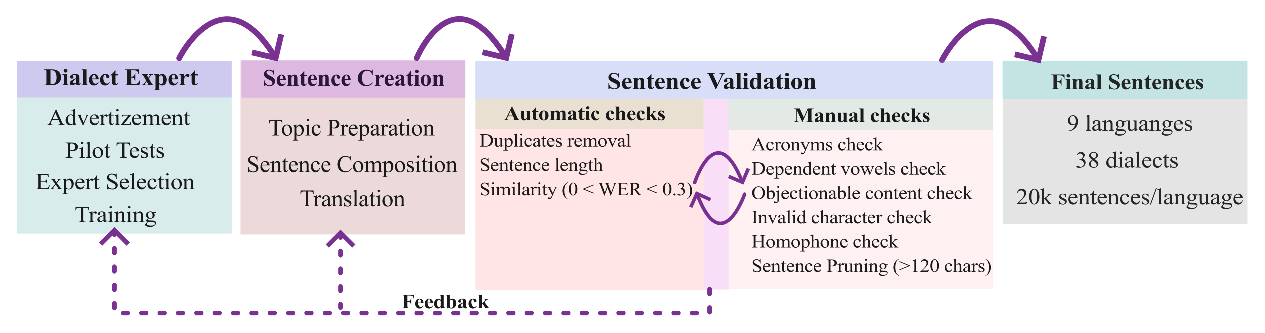
\includegraphics[width=0.9\textwidth]{Styles/figures/figure_2_neurips_v3.eps}
    \caption{Flowchart showing the RESPIN text data preparation.}
    \label{fc1}
\end{figure}

The creation of a dialect-level text corpus was the foundational step in building RESPIN. Figure~\ref{fc1} outlines the overall pipeline. The process began with onboarding and training dialect experts who helped curate text with high dialectal specificity, ensuring the inclusion of regional nuances and speech variation. As discussed earlier, the corpus was designed to collect dialect-rich sentences from agriculture and finance domains -- making RESPIN uniquely domain-specific. Native speakers were hired through a multi-stage selection process to compose these sentences. The raw text was then passed through a validation pipeline combining automatic and manual checks to ensure compliance with linguistic guidelines. Only validated sentences were used in the audio data collection phase.

\subsubsection{Sentence Creation}

While large volumes of digital text exist in standard language formats, they often lack colloquial style and dialectal variation. To address this, RESPIN prioritized sourcing sentences directly from native speakers across districts, ensuring that the text reflects authentic regional expressions and resonates with local speech patterns. Composers were tasked with crafting conversational, domain-specific sentences aligned with designated topics in agriculture and finance. This approach enriched the linguistic diversity of the corpus but also posed challenges, as dialectal variation can differ even within a 5 km radius. Recognizing the fluid and non-standardized nature of dialects, we adopted an inclusive strategy that embraced intra-dialectal variation, resulting in a rich and representative dataset.

Sentence composition followed strict guidelines to ensure consistency and usability: limiting sentence length, avoiding sentence-initial pronouns, excluding non-language numerals, restricting punctuation to full-stop (.), comma (,) and question mark (?), avoiding controversial content, adhering to topic relevance, and maintaining standard acronym formatting. Manual composition was the most accurate but also the most resource-intensive data creation method. While it served as the primary strategy, translation from already composed sentences was used to fill gaps in some dialects. The proportion of translated sentences in Bhojpuri, Chhattisgarhi, Hindi, Kannada, Magahi, Maithili, Marathi, and Telugu was 6.65\%, 100\%, 9.8\%, 0.1\%, 0.4\%, 16.5\%, 5.1\%, and 5.2\%, respectively. Bengali sentences were entirely composed from scratch.

\subsubsection{Sentence Validation}

The raw composed text corpus is passed through a multi-stage validation pipeline involving both automated (AC) and manual checks (MC) by trained language validators. As multiple contributors are involved in sentence composition, inconsistencies and errors are inevitable. Since the corpus is used as stimuli for crowd-sourced audio recording, each sentence must be accurate, unambiguous, coherent, and compatible with the recording interface, making validation essential. The pipeline architecture is largely consistent across languages but includes language-specific adaptations. Key checks include: (1) duplicate removal (AC), (2) invalid character correction (MC), (3) sentence length pruning (MC), (4) acronym standardization (MC), (5) matra correction (MC), (6) word-level edits (MC), (7) similar sentence filtering (MC), (8) homophone disambiguation (MC), and (9) additional language-specific checks (see Appendix~\ref{val_checks}). Approximately 3.6\% of the raw corpus was discarded due to unfixable errors or dialect mismatch. The validation process follows a versioned workflow, where each stage produces a new corpus version to enable rollback and auditing. Independent checks are applied within a single version, while dependent checks are performed sequentially.


% \subsubsection{Sentence Validation}
% To check for errors and perform a quality check, raw composed text corpus is passed through a pipeline consisting of several automated and manual checks by language validators. As the sentences are composed by multiple language personnels, the data at hand is bound to have some errors and deviations from the ideal version. As this text corpus is to be utilized as stimuli for a crowd-sourced recording application for audio data collection, sentences need to be accurate, un-ambiguous, coherent and compatible with the recording application. Thus making the use of the validation pipeline imperative. 

% The validation pipeline consists of several automatic (AC) and manual checks (MC), targeted to specific categories of errors. These categories define the architecture of the validation pipeline, which is almost similar for all languages but is adapted to each language and includes some language-level checks as well. Major categories of checks/errors are: 1) Duplicate sentence removal (AC), 2) Invalid character check and correction (MC), 3) Sentence pruning to specified length (Manual, 4) )Acronyms standardization (MC) 5) Invalid matras' check and correction (MC), 6) Word level check and correction (MC), 7) Similar sentences check (MC), 8) Homophones check (MC) and 9) Various language specific checks (see Appendix~\ref{val_checks} for details). In this validation process, $\sim$3.6\% of raw text corpus, which either didn't belong to the dialect or could not be corrected in accordance with the guidelines.

% Checks in validation pipeline are conducted in a versioning setup i.e., after each set of checks and manual validation, a new version of database is created to maintain backups and history in case of rollbacks in checks. Checks which are independent are done in a single version whereas in case where checks are dependent, they are performed in a sequential manner.

% \subsubsection{Common Sentence Corpus-  NT}
% Need of Common Sentences, their composition and validation process -
% Text data Categorization: Common agriculture, Common banking



% \begin{figure}
%     \centering
%     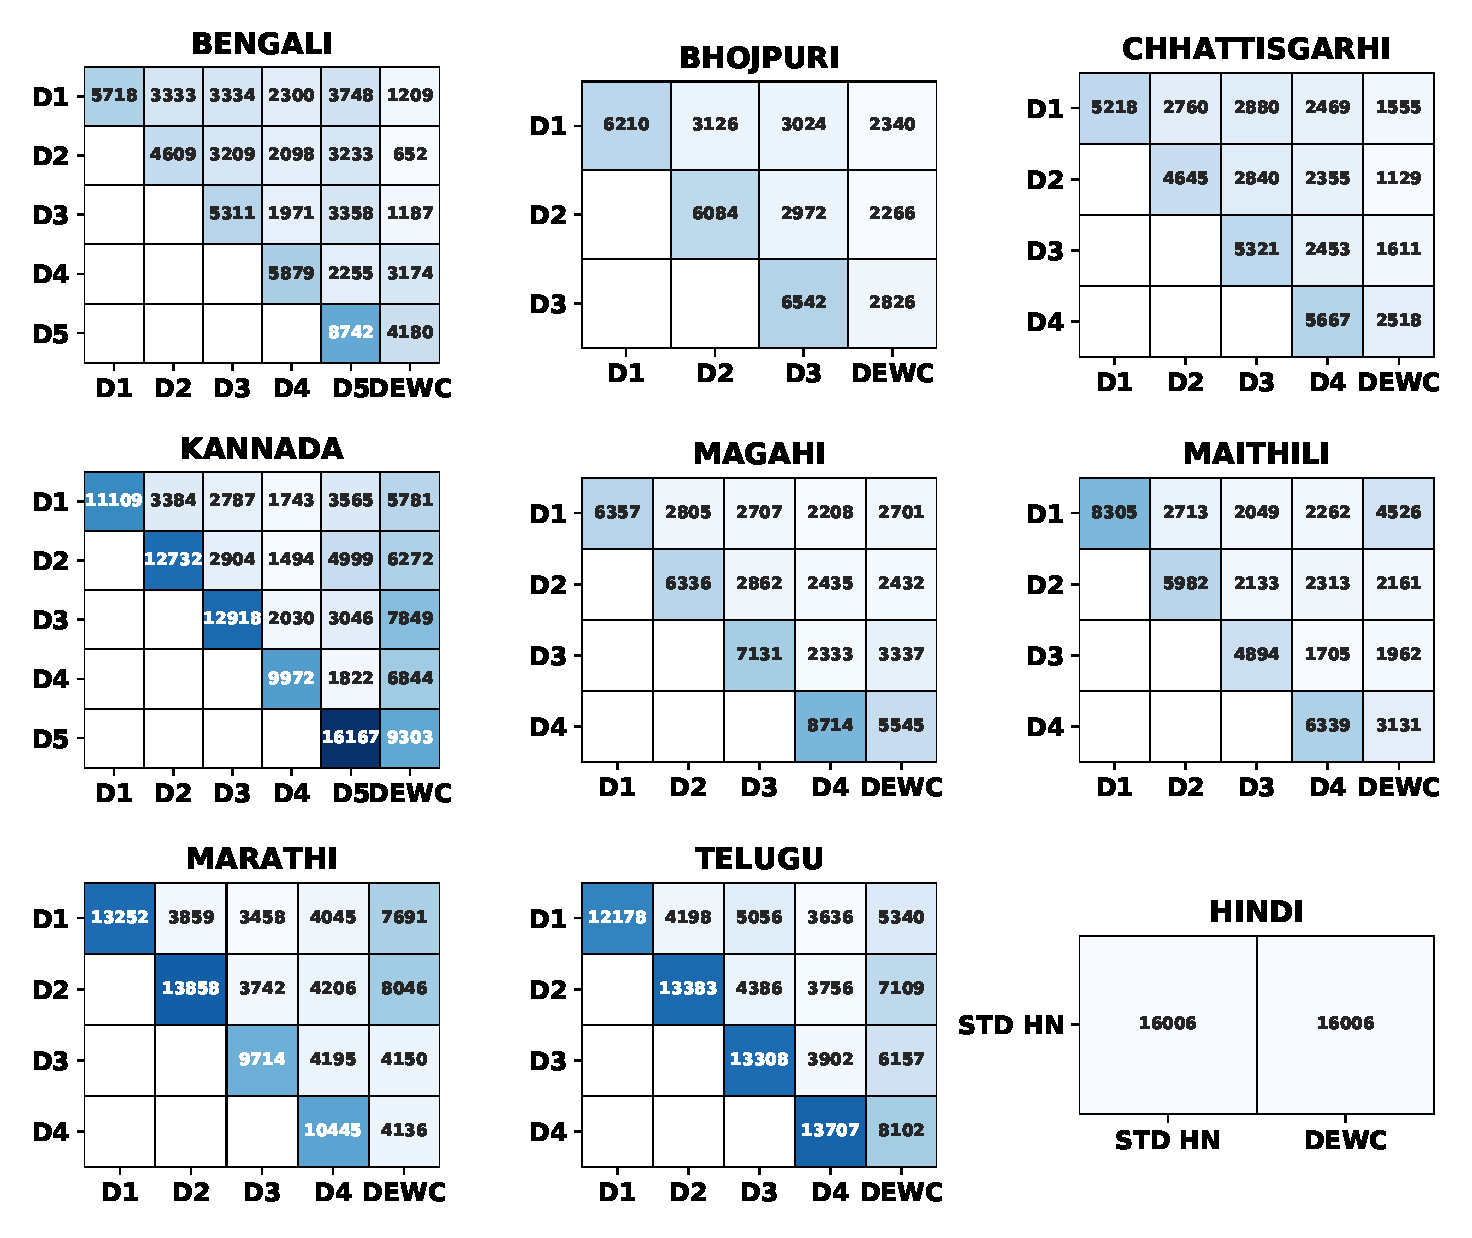
\includegraphics[width=0.9\textwidth]{figures/heatmap_word_analysis.eps}
%     \caption{Unique word distribution and overlap between dialects. Dialect Exclusive Word Count (DEWC) in given in the last column.}
%     \label{word_distribution}
% \end{figure}

% \begin{figure}
%     \centering
%     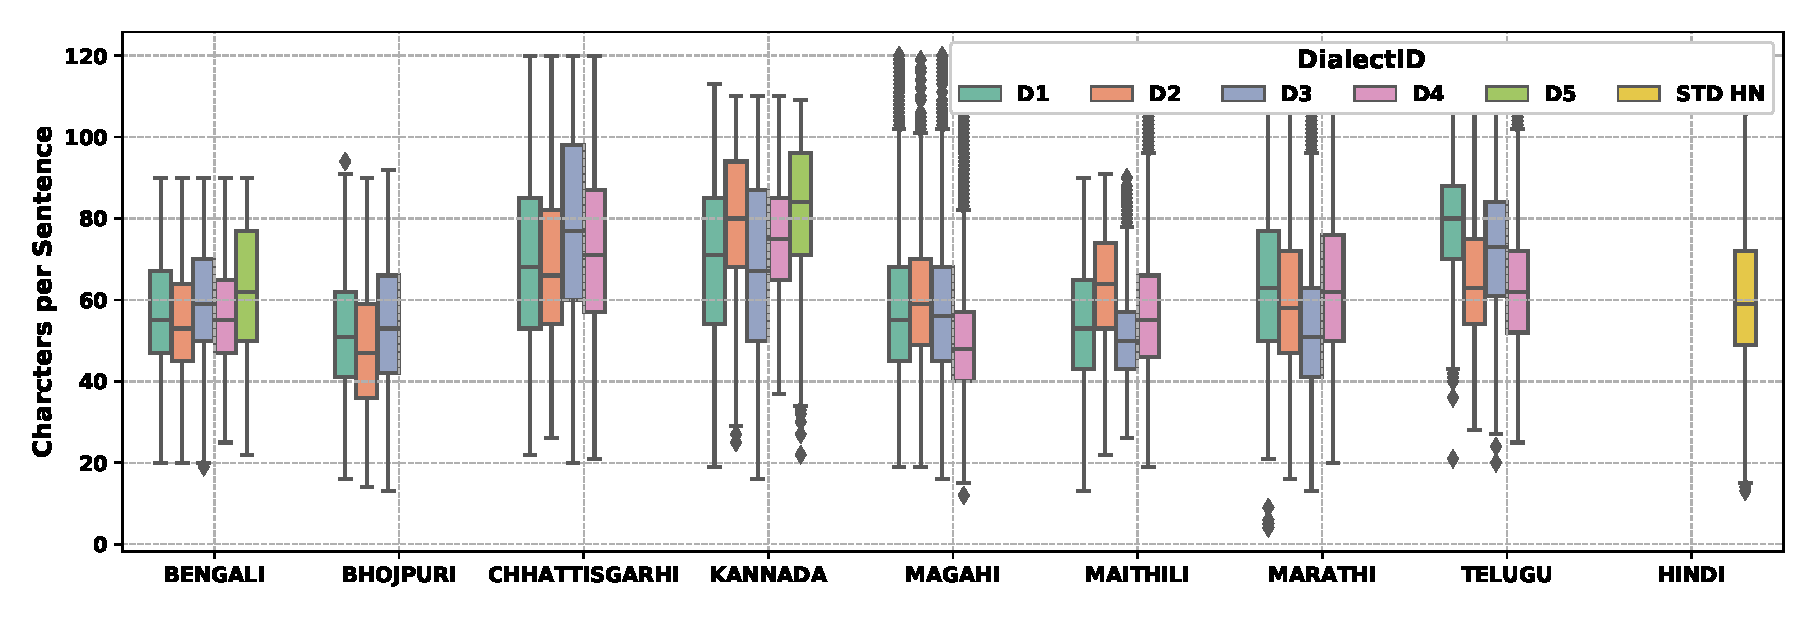
\includegraphics[width=0.9\textwidth]{figures/sentence_len_dist.eps}
%     \caption{Dialect level distribution of characters in a sentence}
%     \label{sent_len_dist}
% \end{figure}

% \subsection{Audio Corpus Creation}

\subsection{Audio Data Acquisition and Validation}

Following the validation of dialect-specific text corpus, audio data collection was conducted via a mobile application. Native speakers of each dialect were prompted to read validated sentences aloud and record them in quiet environments. Each speaker was assigned a maximum of 577 sentences. In some cases, speakers recorded additional sentences to meet dialect-wise targets due to dropouts by other participants. To capture intra-dialectal acoustic variation, each sentence was recorded by multiple speakers -- typically between 30 and 150. This many-to-one sentence-to-speaker mapping enables the corpus to represent diverse pronunciation styles, prosodic patterns, and speech rates within each dialect.

\subsubsection{Audio Validation Pipeline}\label{subsubsec:audio_validation}
The recorded audio data underwent a structured validation pipeline combining manual and semi-automated checks. Initially, approximately 5\% of the utterances in each dialect were manually audited to assess whether the recorded audio matched the corresponding text. Based on this validation, the entire dataset was partitioned into three quality slabs -- \textit{Clean}, \textit{Semi-noisy}, and \textit{Noisy} -- using a semi-automated scoring process.

The slab assignment reflects the proportion of audio-text pairs that are exact matches: the clean slab contains the highest percentage of perfectly aligned utterances, while the noisy slab contains the least. This slab-based categorization allows downstream tasks to select data based on quality requirements and robustness needs. Complete definitions of slabs and associated thresholds are included in the supplementary appendix.

This validation framework ensures that the RESPIN audio corpus is high-quality, dialect-specific, and suitable for benchmarking robust ASR systems under realistic multilingual and multi-dialect conditions.

% %%%%%%%%%%%%%%%%%%%%%%%%%%%%%%%%%%%%%%%%%%%%%%%%%%
% FINAL DATA STATISTICS
% %%%%%%%%%%%%%%%%%%%%%%%%%%%%%%%%%%%%%%%%%%%%%%%%%%
\section{RESPIN-S1.0 Corpus}
\subsection{Text Data Analysis}
\noindent
\begin{minipage}[t]{0.61\textwidth}
  \vspace{0pt}  % Ensures top alignment
  \centering
  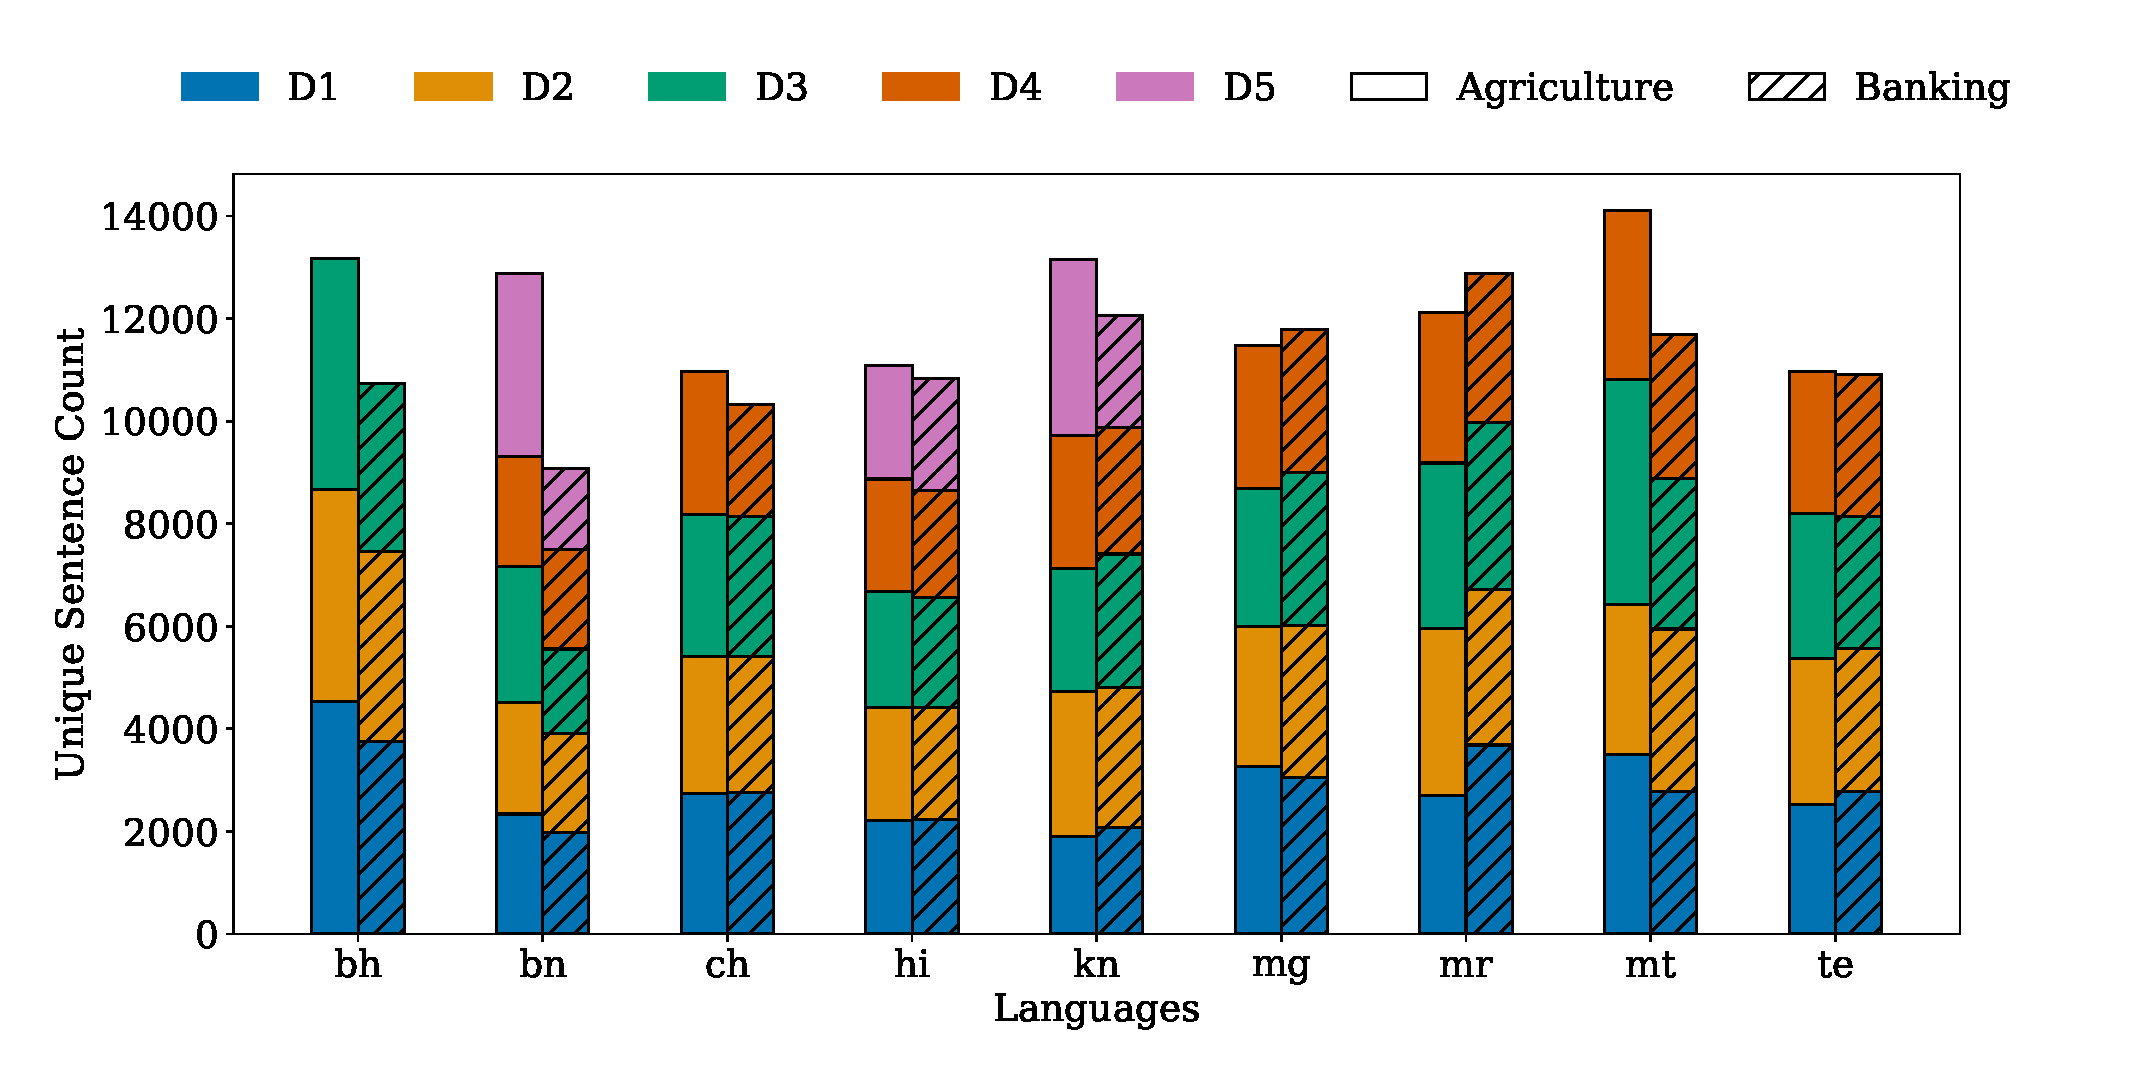
\includegraphics[width=\linewidth]{figures/text_stats/unique_textid_sentence_stats.eps}
  \captionof{figure}{Unique sentence count per dialect, domain and language.}
  \label{fig:sentence_counts}
\end{minipage}%
\hfill
\begin{minipage}[t]{0.37\textwidth}
  \vspace{0pt}  % Ensures top alignment
  \centering
  \captionof{table}{Lexicon statistics across languages.}
  \resizebox{\linewidth}{!}{%
    \begin{tabular}{lrrr}
      \toprule
      \textbf{LID} & \textbf{\#chars} & \textbf{\#phones} & \textbf{\#words} \\
      \midrule
      bn & 64 & 50 & 18571 \\
      bh & 71 & 54 & 14105 \\
      ch & 68 & 50 & 13230 \\
      hi & 72 & 55 & 16571 \\
      kn & 66 & 50 & 50822 \\
      mg & 72 & 54 & 21711 \\
      mt & 72 & 55 & 19336 \\
      mr & 68 & 51 & 35709 \\
      te & 63 & 48 & 39235 \\
      \bottomrule
    \end{tabular}
  }
  \label{tab:lexicon_stats}
\end{minipage}

Figure~\ref{fig:sentence_counts} shows the distribution of unique sentence counts across dialects, domains (Agriculture and Banking), and languages. Each language includes over 20,000 curated sentences across 3-5 dialects, with coverage in both domains per dialect. While perfect balance is constrained by dialect experts' availability and regional factors, the dataset maintains approximate uniformity across dialect-domain pairs. Notable deviations -- e.g., higher contributions from dialect D5 in \texttt{kn} and D3 in \texttt{mt} -- likely reflect stronger regional participation or easier contributor access.

Table~\ref{tab:lexicon_stats} reports lexicon statistics, including unique characters, phonemes, and words per language. Lexicons are derived from the full sentence set. Kannada (\texttt{kn}) and Telugu (\texttt{te}) show higher word counts (50k and 39k+), indicative of richer morphology and larger text pools. In contrast, Bhojpuri (\texttt{bh}) and Chhattisgarhi (\texttt{ch}) have more compact vocabularies, possibly due to lower lexical variation. Character counts (63-72) align with script complexity, and phoneme inventories (≈50-55) match known Indo-Aryan and Dravidian phonological structures.

Together, these statistics reflect the linguistic richness and dialectal coverage of the text corpus. The balance across dialects and domains, combined with diverse lexicons, makes the dataset a strong foundation for multilingual and multidialectal ASR, language modeling, and speech-language technology research.




\subsection{Audio Data Analysis}
\subsubsection{Slab-Wise Audio Distribution}\label{sec:slabwise_distribution}

\begin{table}[t]
\centering
\caption{Dialect-wise duration (in hours) across Clean, Semi-noisy, and Noisy subsets for 9 Indian languages.}
\label{tab:duration_updated}
\begin{adjustbox}{width=0.85\textwidth}
\begin{tabular}{llrrrrrrrrr}
\toprule
\textbf{Dialect} & \textbf{Type} & \textbf{bh} & \textbf{bn} & \textbf{ch} & \textbf{hi} & \textbf{kn} & \textbf{mg} & \textbf{mr} & \textbf{mt} & \textbf{te} \\
\midrule
\multirow{3}{*}{D1} & Clean       & 351.25 & 206.40 & 344.89 & 205.25 & 237.38 & 340.88 & 312.58 & 195.10 & 348.78 \\
                    & Semi-noisy  &  32.09 &  64.61 &  31.75 &  49.35 &  58.72 &  15.12 &  63.69 & 117.80 &  51.61 \\
                    & Noisy       &  41.43 &   1.31 &  21.07 &  80.67 &  52.81 &  17.60 &  61.15 &  71.01 &  41.96 \\
\midrule
\multirow{3}{*}{D2} & Clean       & 417.74 & 271.45 & 329.20 & 159.78 & 245.03 & 349.01 & 328.89 & 112.16 & 333.28 \\
                    & Semi-noisy  &  11.25 &  12.97 &  22.37 &  90.78 &  37.07 &  13.94 &  54.39 & 139.60 &  74.12 \\
                    & Noisy       &   5.68 &   0.80 &  12.07 &  88.07 &  38.36 &  13.13 &  49.17 & 180.44 &  33.67 \\
\midrule
\multirow{3}{*}{D3} & Clean       & 347.97 & 283.17 & 297.63 & 195.93 & 235.92 & 333.33 & 321.62 & 203.16 & 331.65 \\
                    & Semi-noisy  &  62.53 &  22.55 &  77.19 &  70.51 &  55.35 &  26.11 &  60.99 & 164.29 &  58.34 \\
                    & Noisy       &  29.46 &   1.10 &  22.81 &  68.28 &  44.17 &  14.87 &  23.49 &  55.73 &  54.49 \\
\midrule
\multirow{3}{*}{D4} & Clean       &    --  & 216.14 & 324.25 & 138.83 & 248.10 & 321.18 & 316.39 & 212.64 & 290.27 \\
                    & Semi-noisy  &    --  &  62.64 &  67.56 & 116.41 &  34.66 &  57.22 & 156.14 &  88.55 &  38.46 \\
                    & Noisy       &    --  &   2.13 &  34.17 &  99.35 &  48.41 &  27.14 &  66.13 &  98.11 &  18.87 \\
\midrule
\multirow{3}{*}{D5} & Clean       &    --  & 236.08 &    --  & 245.14 & 228.13 &    --  &    --  &    --  &    --  \\
                    & Semi-noisy  &    --  &  27.19 &    --  &  35.74 &  64.40 &    --  &    --  &    --  &    --  \\
                    & Noisy       &    --  &   1.39 &    --  &  54.49 &  42.48 &    --  &    --  &    --  &    --  \\
\midrule
\textbf{Total} & Clean      & 1116.96 & 1213.24 & 1295.97 & 944.93 & 1194.56 & 1344.40 & 1279.48 & 723.06 & 1303.98 \\
\textbf{Total} & Semi-noisy &  105.87 &  189.96 &  198.87 & 362.79 &  250.20 &  112.39 &  335.21 & 510.24 &  222.53 \\
\textbf{Total} & Noisy      &   76.57 &    6.73 &   90.12 & 390.86 &  226.23 &   72.74 &  199.94 & 405.29 &  148.99 \\
\bottomrule
\end{tabular}
\end{adjustbox}
\end{table}

Table~\ref{tab:duration_updated} summarizes dialect-wise audio durations (in hours) across the Clean, Semi-noisy, and Noisy slabs for all nine Indian languages. The full corpus contains over 12,000 hours of read-speech audio, covering more than 20,000 sentences per language. Based on transcription quality and alignment confidence (see Section~\ref{subsubsec:audio_validation}), audio is grouped into three slabs: \textit{Clean}, \textit{Semi-noisy}, and \textit{Noisy}.

The intended target was 200 hours of Clean data per dialect for languages with five dialects (e.g., Hindi, Bengali, Kannada), and 250 hours per dialect for those with four dialects (e.g., Magahi, Marathi, Telugu). While most dialects met this target -- particularly in Bengali, Chhattisgarhi, Kannada, and Marathi -- some under-resourced dialects (e.g., Hindi D2, D4 and Maithili D2) fell short, requiring larger proportions of \textit{Semi-noisy} and \textit{Noisy} data to ensure sufficient representation. Such shortfalls are likely due to challenges in recruiting fluent readers in specific dialects, influenced by literacy, regional accessibility, and dialectal overlap. For example, Maithili and Hindi have lower \textit{Clean}-slab totals -- 723.06 and 944.93 hours respectively -- compared to other languages that exceed 1100 hours.

Across the full dataset, the \textit{Clean} slab comprises 10,416.58 hours, \textit{Semi-noisy} 2,288.06 hours, and \textit{Noisy} 1,617.47 hours. The inclusion of noisy data captures realistic transcription variability and supports ASR training under practical conditions.

This slab-wise stratification balances dialectal coverage with data quality, enabling robust model evaluation under varying transcription conditions -- essential for developing dialect-aware ASR systems.

\subsubsection{Signal-Level Audio Quality}
\begin{table}[th!]
\centering
\caption{Audio statistics per language including low SNR and speaking rate.}
\label{tab:audio_stats}
\begin{adjustbox}{width=0.6\textwidth}
\begin{tabular}{lrrrrrrr}
\toprule
\textbf{LID} & \textbf{\#Files} & \textbf{\#Low SNR} & \textbf{\%SNR} & \textbf{Wds/Aud} & \textbf{Dur (s)} & \textbf{WPM} \\
\midrule
bn & 870{,}793    & 3712 & 0.43 &  9 & 4.18 & 142.00 \\
bh & 866{,}619    & 4404 & 0.51 & 10 & 3.94 & 159.37 \\
ch & 823{,}803    & 1605 & 0.19 & 12 & 4.87 & 161.18 \\
hi & 756{,}886    & 1686 & 0.22 & 11 & 3.81 & 173.91 \\
kn & 744{,}617    & 1749 & 0.23 &  8 & 4.84 & 110.16 \\
mg & 968{,}365    & 2981 & 0.31 & 10 & 4.25 & 153.97 \\
mt & 518{,}504    & 1144 & 0.22 & 10 & 3.87 & 150.73 \\
mr & 1{,}002{,}599 & 2055 & 0.20 &  8 & 4.27 & 132.66 \\
te & 895{,}131    & 3051 & 0.34 &  8 & 4.40 & 117.16 \\
\bottomrule
\end{tabular}
\end{adjustbox}

\vspace{4pt}
\noindent
\textbf{Abbreviations:} LID = Language ID; \#Files = No. of audio files; \#Low SNR = No. of low-SNR files (SNR < 4 dB); \%SNR = Percentage of low-SNR files;  
Wds/Aud = Avg. words per audio; Dur (s) = Avg. duration in seconds; WPM = Words per minute.
\vspace{-5mm}
\end{table}

Table~\ref{tab:audio_stats} presents signal-level audio quality metrics for \textit{Clean}-slab across languages, including the number and percentage of low-SNR files, average words per audio, average duration, and speaking rate in words per minute (WPM). To ensure accurate measurements, each audio was trimmed using forced alignment timestamps to remove leading and trailing noise or prompts. SNR was computed using the pre-trained FB-Denoiser~\cite{defossez2020real}, with 4 dB empirically chosen as the threshold for classifying low-SNR files. Speaking rate was calculated as the ratio of transcript word count to the forced-alignment-based audio duration. Overall, low-SNR files make up less than 1\% of the data in all languages, confirming high acoustic quality. WPM values range from 110 to 174, with lower rates observed for Kannada and Telugu due to their agglutinative linguistic structure, which results in longer word durations.%\vspace{-3mm}

\subsubsection{Speaker Metadata Validation}\label{sec:spk_meta}

To assess the correctness and consistency of speaker metadata, we designed two validation checks: (1) intra-speaker and (2) inter-speaker. The intra-speaker check identifies inconsistencies within a single speaker’s recordings, while the inter-speaker check detects if recordings assigned to different speaker IDs may actually belong to the same individual. To address these inconsistencies, we developed a bucketization algorithm, which was evaluated on unseen data (see Appendix~\ref{sec:spk_bucket} for details). The method successfully resolved 99.28\% of intra-speaker issues and 52.91\% of inter-speaker mismatches, providing a reliable approximation of speaker identity consistency within the corpus. Following the speaker bucketization check, a subset of speakers with no intra- or inter-speaker discrepancies was identified and used to prepare the development and test sets, ensuring no speaker overlap across train, dev, and test splits.

\section{Benchmarking ASR Performance}
\label{asr_performance}\vspace{-3mm}

\subsection{Datasets}
\begin{table}[t]
\centering
\caption{Train, development, and test set statistics for each language.}
\label{tab:split_stats}
\resizebox{\textwidth}{!}{%
\begin{tabular}{l|c|rrrr|rrrr|rrrr}
\toprule
\multirow{2}{*}{\textbf{LID}} & \multirow{2}{*}{\textbf{\#Dialects}} 
& \multicolumn{4}{c|}{\textbf{Train Set}} 
& \multicolumn{4}{c|}{\textbf{Dev Set}} 
& \multicolumn{4}{c}{\textbf{Test Set}} \\
\cmidrule(lr){3-6} \cmidrule(lr){7-10} \cmidrule(lr){11-14}
 & & Dur (h) & \#Utts & \#Sents & \#Spks 
   & Dur (h) & \#Utts & \#Sents & \#Spks 
   & Dur (h) & \#Utts & \#Sents & \#Spks \\
\midrule
bh & 3 & 142.98 & 95280 & 19056 & 1445 & 2.14 & 1500 & 575 & 60  & 3.10 & 2220 & 694 & 120 \\
bn & 5 & 142.96 & 85800 & 17160 & 1280 & 2.27 & 1500 & 494 & 100 & 3.26 & 2174 & 648 & 200 \\
ch & 4 & 175.22 & 85800 & 17160 & 1586 & 2.40 & 1413 & 511 & 80  & 3.85 & 2234 & 695 & 160 \\
hi & 5 & 128.47 & 85800 & 17160 & 2172 & 2.21 & 1539 & 722 & 100 & 3.30 & 2288 & 853 & 201 \\
kn & 5 & 164.83 & 85800 & 17160 & 1859 & 2.37 & 1430 & 518 & 100 & 3.61 & 2161 & 663 & 200 \\
mg & 4 & 157.77 & 95280 & 19056 & 1493 & 2.10 & 1431 & 494 & 80  & 3.17 & 2193 & 640 & 160 \\
mt & 4 & 159.32 & 95280 & 19056 & 1913 & 2.06 & 1409 & 693 & 80  & 3.33 & 2172 & 993 & 160 \\
mr & 4 & 140.49 & 95280 & 19056 & 2305 & 1.98 & 1386 & 509 & 80  & 3.04 & 2170 & 711 & 160 \\
te & 4 & 155.89 & 95280 & 19056 & 1848 & 2.30 & 1438 & 500 & 80  & 3.37 & 2226 & 652 & 160 \\
\bottomrule
\end{tabular}%
}
% \vspace{1mm}
\begin{minipage}{\textwidth}
\footnotesize
\textbf{LID}: Language ID, \textbf{\#Dialects}: number of dialects, \textbf{Dur}: duration in hours, 
\textbf{\#Utts}: number of utterances, \textbf{\#Sents}: number of unique sentences, \textbf{\#Spks}: number of speakers.
\end{minipage}\vspace{-5mm}
\end{table}

To support reproducible research and enable fair benchmarking, we release standardized train, development, and test splits for each of the nine languages in the RESPIN corpus.\footnote{RESPIN-S1.0 data is available at: \url{https://github.com/saurabhk0317/respin_data_neurips25}} Table~\ref{tab:split_stats} summarizes split statistics, including duration, number of utterances, unique sentences, and speakers. Each language contains 3–5 dialects and 130–175 hours of training audio comprising 85k–95k utterances. The dev and test sets include 2–4 hours of speech each, with up to 2.2k utterances from 60–200 distinct speakers. The train set shown in Table~\ref{tab:split_stats} refers to the \textit{small} train set, a balanced subset of the \textit{clean} corpus used for all ASR experiments in this paper. For \texttt{mt\_D2}, where clean audio was insufficient, a small portion of semi-noisy data was included. Detailed statistics for other training variants are provided in the supplementary appendix.

All dev and test sets consist exclusively of speakers from the \textit{uncontaminated} bucket (Section~\ref{sec:spk_meta}), ensuring high-quality evaluation without speaker overlap across splits. The splits are carefully constructed to preserve dialectal diversity, balance sentence types, and maintain speaker disjointness—providing a reliable foundation for evaluating both traditional ASR systems and fine-tuned pretrained models.

% \subsection{Existing ASR models}
% % Sathvik
% \subsection{Experimental setup}
% \subsubsection{Whisper models}
% % We fine-tune OpenAI's Whisper models, which are encoder-decoder-based multilingual ASR models, to adapt them to our specific training set and evaluate their performance on a designated test set. 
% We fine-tune OpenAI's Whisper models, which are encoder-decoder-based multilingual ASR models pre-trained on a large corpus of supervised and weakly supervised audio-text pairs. These models demonstrate robust performance across diverse languages and noisy acoustic conditions. In our work, we adapt them to a domain-specific training set and evaluate their effectiveness on a designated test set to assess performance improvements and generalization to the target task. For our experiments, we utilize three variants of the Whisper model: tiny (39M parameters), base (74M parameters) and small (244M parameters). The pre-trained versions of these models, accessible on Hugging Face\footnote{\url{https://huggingface.co/}}, serve as the initialization point for fine-tuning. The training is conducted on a single NVIDIA GeForce RTX 3090 GPU using Hugging Face's Trainer framework with default hyperparameters. The batch size is adjusted dynamically based on the maximum capacity the GPU can handle. We employ early stopping based on the Word Error Rate (WER) of the validation set to prevent overfitting. Fine-tuning is performed separately for each language, and decoding on the test set incorporates language IDs to enhance accuracy.

% \subsubsection{Fairseq models}
% \textit{\textbf{IndicWav2Vec}}\newline
% The IndicWav2Vec2 model is a multilingual speech model developed by AI4Bharat\footnote{https://ai4bharat.iitm.ac.in/}. It's a SSL model for Indian languages trained on a diverse corpus of speech data encompassing 40 Indian languages from 4 different language families.The model is based on the Wav2Vec 2.0 framework, which uses a transformer-based encoder for learning speech representations, It aims to enhance ASR tasks with robust performance.\newline\newline
% \textit{\textbf{SPRING-INX SSL Wav2Vec2}}\newline
% The SPRING-INX SSL Wav2Vec2 model is a self-supervised learning (SSL) model developed by the SPRING Lab\footnote{https://asr.iitm.ac.in/} Indian Institute of Technology (IIT) Madras. The model is based on the Wav2Vec 2.0 framework, which uses a transformer-based encoder for learning speech representations trained on 30,000 hours of raw speech data across 24 Indian languages.\newline\newline
% \textit{\textbf{SPRING-INX SSL Data2Vec\_AQC}}\newline
% The SPRING-INX SSL Data2Vec\_AQC model is a self-supervised learning (SSL) model developed by the SPRING Lab Indian Institute of Technology (IIT) Madras. The model is based on the data2vec framework, incorporating modules for data augmentations, quantized representations, and clustering. Trained on a large corpus of speech data, leveraging both unlabeled and limited labeled data.
% \subsubsection{ESPnet models}
% \textit{\textbf{e-branchformer}}\newline
% \textbf{Experimental Setup}

\subsection{Existing ASR Models}

We evaluate a variety of ASR models ranging from traditional models trained from scratch to modern self-supervised and multilingual pretrained models. These include Kaldi and ESPnet-based models trained on RESPIN data, as well as pretrained models like Whisper, IndicWav2Vec, and SPRING SSL models. Fine-tuning is performed wherever applicable to enable fair comparison across architectures and training paradigms.

\subsection{Experimental Setup}\vspace{-3mm}

All model training and fine-tuning experiments were performed on a single NVIDIA RTX 3090 GPU with 24GB memory.

\textbf{Whisper Models:} We fine-tune the Tiny (39M), Base (74M), and Small (244M) variants using Hugging Face checkpoints and the Trainer API with default settings. Fine-tuning is done separately for each language with early stopping based on validation WER. Language IDs are passed during decoding.

\textbf{Fairseq Models:} We fine-tune three SSL models on RESPIN: (i) IndicWav2Vec (trained on 40 Indian languages)\footnote{\url{https://github.com/AI4Bharat/IndicWav2Vec}}, (ii) SPRING-Wav2Vec2 (30k hours, 24 languages), and (iii) SPRING-Data2Vec-AQC, which incorporates augmentation, quantization, and clustering\footnote{\url{https://asr.iitm.ac.in/models}}.

\textbf{ESPnet Models:} We train a CTC-Attention hybrid model with an \texttt{e\_branchformer} encoder (8 blocks, 256-dim hidden units) using Adam optimizer, SpecAugment, mixed-precision (AMP), and early stopping with patience 5 based on validation CER.

\textbf{Kaldi Models:} We train TDNN-HMM models using the standard chain recipe with 40-dim MFCCs, iVectors, speed/volume perturbation, and a tri-gram LM trained on RESPIN transcripts.

Pretrained models and training recipes for Whisper, Fairseq, and ESPnet experiments are available at: \url{https://github.com/labspire/respin_baselines}\footnote{\url{https://github.com/labspire/respin_baselines}}.


% \subsection{Experimental Setup}\vspace{-3mm}

% \textbf{Whisper Models:} We fine-tune OpenAI’s Whisper models (Tiny: 39M, Base: 74M, Small: 244M), pre-trained on large multilingual audio-text corpora. Checkpoints are initialized from Hugging Face. Fine-tuning is done separately for each language using Hugging Face’s Trainer API with default hyperparameters. Training is performed on a single NVIDIA RTX 3090 GPU with dynamic batch sizing. Early stopping is based on validation WER. Language IDs are passed during decoding to aid recognition.

% \textbf{Fairseq Models:} We evaluate three self-supervised models: (i) \textit{IndicWav2Vec}, trained on 40 Indian languages using the Wav2Vec 2.0 framework; (ii) \textit{SPRING-Wav2Vec2}, trained on 30k hours across 24 Indian languages; and (iii) \textit{SPRING-Data2Vec-AQC}, which incorporates data augmentation, quantization, and clustering into the Data2Vec architecture. All models are fine-tuned on RESPIN subsets using Fairseq.

% \textbf{ESPnet Models:} We train a Conformer-style model using ESPnet’s \texttt{e\_branchformer} encoder with 8 blocks, 256-dim hidden states, 4 attention heads, and relative positional encodings. Training is conducted on a single NVIDIA 3090 GPU (24GB) for 70 epochs with Adam optimizer (lr = 0.002, weight decay = $1e^{-6}$), label smoothing (0.1), and SpecAugment. Batch size is defined by number of elements (16M bins), with gradient accumulation every 4 steps. Mixed-precision training (AMP) is enabled. Validation is based on CER from the CTC branch.

% \textbf{Kaldi Models:} We train TDNN-HMM models on RESPIN using the standard chain model recipe. Features include 40-dim MFCCs and iVectors. Speed and volume perturbation are used for data augmentation. Decoding uses a pruned first-pass graph and tri-gram language model trained on RESPIN transcripts. Final scoring follows standard Kaldi procedures.

\subsection{Results and discussion}
\begin{table}[t]
\centering
\caption{CER and WER (\%) for different models across languages. \textbf{Pretrained models} refer to models fine-tuned on publicly available data other than RESPIN. \textbf{Traditional models} are trained from scratch on RESPIN. \textbf{Fine-tuned models} are pretrained SSL or Whisper models further fine-tuned on a subset of RESPIN. For SeamlessM4T-v2-Large, \textbf{bh}, \textbf{ch}, and \textbf{mg}, and for the pretrained SSL models, \textbf{bh}, \textbf{ch}, \textbf{mg}, and \textbf{mt} are evaluated using Hindi-tuned models.}\vspace{3pt}
\label{tab:baseline_results}
\resizebox{\textwidth}{!}{%
\begin{tabular}{l|rrrrrrrrrr|rrrrrrrrrr}
\toprule
\multirow{2}{*}{\textbf{Model}} 
& \multicolumn{10}{c|}{\textbf{CER (\%)}} 
& \multicolumn{10}{c}{\textbf{WER (\%)}} \\
\cmidrule(lr){2-11} \cmidrule(lr){12-21}
& \textbf{bh} & \textbf{bn} & \textbf{ch} & \textbf{hi} & \textbf{kn} & \textbf{mg} & \textbf{mr} & \textbf{mt} & \textbf{te} & \textbf{avg}
& \textbf{bh} & \textbf{bn} & \textbf{ch} & \textbf{hi} & \textbf{kn} & \textbf{mg} & \textbf{mr} & \textbf{mt} & \textbf{te} & \textbf{avg} \\
\midrule

\rowcolor{gray!10}
\multicolumn{21}{l}{\textbf{Pretrained Models (fine-tuned on non-RESPIN public data)}} \\
SeamlessM4T-v2-Large       & 29.09 & 17.54 & 33.20 & 15.34 & 18.91 & 30.07 & 14.44 & 27.15 & 14.33 & 22.23 & 56.77 & 45.56 & 71.86 & 25.43 & 55.38 & 56.49 & 42.09 & 66.64 & 46.11 & 51.81 \\
IndicW2V                  & 17.08 & 14.27 & 22.77 & 11.02 & 10.37 & 19.64 & 15.09 & 23.30 & 8.61  & 15.80 & 51.61 & 42.83 & 65.98 & 28.34 & 42.37 & 54.32 & 53.91 & 66.10 & 37.82 & 49.25 \\
SPRING-W2V2                & 15.10 & 12.50 & 20.81 & 8.80  & 11.43 & 16.35 & 7.56  & 20.12 & 6.97  & 13.29 & 41.32 & 25.93 & 55.42 & 22.99 & 44.35 & 42.09 & 34.15 & 53.69 & 36.32 & 39.58 \\
SPRING-Data2Vec-AQC        & 15.02 & 11.94 & 21.26 & 7.20  & 10.78 & 15.81 & 7.49  & 19.91 & 6.53  & 12.88 & 42.35 & 23.69 & 56.17 & 20.93 & 42.79 & 42.47 & 33.40 & 53.65 & 33.98 & 38.83 \\
\addlinespace

\rowcolor{gray!10}
\multicolumn{21}{l}{\textbf{Traditional Models (trained from scratch on RESPIN subset)}} \\
TDNN-HMM                        & 5.67  & 5.22  & 4.45  & 3.25  & 4.88  & 7.69  & 3.30  & 6.53  & 3.94  & 4.99  & 17.57 & 16.87 & 12.69 & 8.72  & 23.01 & 22.33 & 13.40 & 20.13 & 20.81 & 17.28 \\
E-Branchformer                  & 4.95  & 4.33  & 3.63  & 3.52  & 4.62  & 6.68  & 3.19  & 5.75  & 3.97  & 4.52  & 15.21 & 14.96 & 10.59 & 9.94  & 24.50 & 20.38 & 14.48 & 17.95 & 21.64 & 16.63 \\
\addlinespace

\rowcolor{gray!10}
\multicolumn{21}{l}{\textbf{Fine-tuned Models (fine-tuned on RESPIN subset)}} \\
Whisper-Tiny                    & 9.62  & 11.60 & 7.13  & 9.69  & 12.62 & 13.98 & 9.15  & 10.73 & 11.43 & 10.66 & 27.45 & 32.51 & 20.81 & 21.71 & 48.54 & 36.40 & 30.93 & 31.96 & 41.61 & 32.44 \\
Whisper-Base                    & 7.15  & 7.69  & 5.36  & 5.80  & 8.10  & 10.44 & 6.23  & 7.51  & 7.51  & 7.31  & 22.51 & 24.71 & 16.67 & 15.19 & 36.52 & 30.54 & 24.28 & 24.80 & 32.99 & 25.36 \\
Whisper-Small                   & 7.90  & 5.46  & 3.85  & 4.16  & 6.00  & 7.46  & 3.93  & 5.94  & 6.54  & 5.69  & 19.02 & 18.91 & 12.36 & 11.78 & 29.66 & 23.94 & 16.95 & 20.28 & 27.82 & 20.08 \\
IndicW2V                   & 4.42  & 4.28  & 3.24  & 3.16  & 4.68  & 6.02  & 3.19  & 5.19  & 4.54  & 4.30  & 16.07 & 16.65 & 11.36 & 10.47 & 24.86 & 21.51 & 15.13 & 19.19 & 24.03 & 17.69 \\
SPRING-W2V2                & 3.92  & 3.86  & 2.99  & 2.37  & 4.30  & 5.20  & 2.49  & 4.37  & 3.85  & 3.71  & 14.61 & 15.12 & 10.74 & 8.22  & 23.90 & 19.40 & 12.75 & 16.64 & 21.92 & 15.92 \\
SPRING-Data2Vec-AQC        & 3.95  & 3.63  & 2.84  & 2.27  & 4.11  & 4.98  & 2.38  & 4.30  & 3.72  & 3.58  & 14.84 & 14.15 & 10.25 & 7.91  & 23.13 & 18.50 & 12.28 & 16.41 & 21.17 & 15.40 \\

\bottomrule
\end{tabular}
}\vspace{-5mm}
\end{table}

% \section{Discussion}

Table~\ref{tab:baseline_results} presents the ASR performance of various models on nine Indian languages using the RESPIN corpus. The results highlight the importance of dialectal supervision in training and fine-tuning ASR models.

\textbf{Pretrained models struggle without dialectal supervision:}
Models pretrained on external corpora -- such as SeamlessM4T-v2-Large, IndicW2V2 (PT), and SPRING-W2V2 (PT) -- perform poorly across most languages. Their high WERs, exceeding 50\% in some cases, reflect the lack of dialectal variation in the training data. Performance drops are especially evident for dialect-heavy languages like Bhojpuri and Chhattisgarhi.

\textbf{Training from scratch on RESPIN improves performance:}
Traditional models such as TDNN-HMM and E-Branchformer, trained entirely on RESPIN subsets, significantly outperform the pretrained models. E-Branchformer achieves an average WER of 16.63\%, underscoring the benefits of dialect-specific supervision even without large-scale pretraining.

\textbf{Whisper fine-tuning offers limited gains:}
While Whisper models (Tiny, Base, Small) fine-tuned on RESPIN perform better than their pretrained-only versions, they still lag behind scratch-trained models. Whisper-Small, for instance, shows higher WER than E-Branchformer despite using the same data, suggesting that general-purpose multilingual models do not fully adapt to dialectal variation.

\textbf{SSL models fine-tuned on RESPIN perform best:}
Self-supervised models like SPRING-W2V2 and SPRING-Data2Vec-AQC, when fine-tuned on RESPIN, outperform all other approaches. SPRING-Data2Vec-AQC achieves the lowest average WER (15.40\%) and delivers the best performance across most individual languages, demonstrating the strength of combining SSL pretraining with dialect-aware fine-tuning.

\textbf{Summary:}
These findings show that RESPIN’s dialectal coverage provides clear benefits across model types. Pretrained models struggle with domain mismatch, while both scratch-trained and fine-tuned models gain significantly from RESPIN’s diversity. Fine-tuned SSL models emerge as the most effective strategy for multi-dialect ASR in the Indian context.\vspace{-3mm}

\section{Applications, Impact, and Limitations}

RESPIN-S1.0 has already made a tangible impact within the speech technology community. Over the past two years, subsets of the corpus have been released through various workshops and challenges. A subset of Bengali and Bhojpuri data was used in the SLT Code Hackathon 2022 to build dialectal ASR systems. The first Multi-Dialect ASR Challenge (MADASR) was held at ASRU 2023~\cite{Udupa_ASRU23,Tanel_ASRU23} using RESPIN data for Bengali and Bhojpuri, and the ongoing MADASR 2.0 Challenge at ASRU 2025 expands this to 1,200 hours across eight languages (bh, bn, ch, kn, mg, mr, mt, te), enabling large-scale benchmarking of dialect-aware ASR systems. RESPIN has also been used to study dialect identification performance across eight Indian languages~\cite{Amartyaveer_ICASSP25}. Beyond ASR, the corpus supports a range of tasks including language and dialect identification (LID/DID), unsupervised speech translation, and broader speech-language research, particularly for underrepresented Indian languages and domain-specific applications. However, RESPIN-S1.0 has some limitations. It currently contains only read speech, while spontaneous or conversational data is often more representative of real-world scenarios. It is also limited to two domains- agriculture and finance- selected for societal relevance; expanding to domains such as healthcare and education could enhance applicability. Finally, while efforts were made to ensure inclusivity, the reliance on literate native speakers with mobile access may underrepresent the most marginalized populations. Nevertheless, RESPIN sets a strong foundation for inclusive and dialect-rich ASR development in India, and future versions will address these limitations through broader linguistic coverage and inclusion of spontaneous speech.\vspace{-3mm}

\section{Conclusion and Future Work}

RESPIN-S1.0 is the first large-scale, publicly available corpus that combines dialectal and domain coverage across nine Indian languages, including low-resource ones like Bhojpuri, Chhattisgarhi, and Magahi. By addressing long-standing gaps in linguistic diversity, speaker variation, and domain relevance, RESPIN enables the development of more inclusive and robust speech technologies for Indian languages. The standardized benchmarks, metadata, and carefully curated splits provided with this release support reproducible research in ASR and beyond. As part of ongoing efforts, RESPIN-S2.0 will expand to cover additional languages, dialects, spontaneous speech, and new domains. We invite researchers, institutions, and industry collaborators to join us in building the next generation of speech and language tools that reflect the full diversity of India's linguistic landscape.\vspace{-3mm}


\section*{Acknowledgements}

This work was supported by the Bill and Melinda Gates Foundation. We thank the many NGOs, volunteers, and contributors who participated in data collection, validation, and community engagement -- both online and offline. Their efforts were instrumental in making RESPIN-S1.0 possible.

% \section*{References}
\bibliographystyle{unsrt}
\bibliography{respin_references}

\newpage
\appendix

\section{Text Data Creation and Validation Details}
\subsection{Detailed Text Validation Checks}
\label{val_checks}

The following checks were implemented as part of the text validation pipeline. These include a combination of automatic and manual steps designed to ensure that the composed text adheres to the required linguistic, formatting, and usability standards across all dialects.

\begin{enumerate}
    \item \textbf{Duplicate Sentence Removal (Automatic)} \\
    A pairwise Word Error Rate (WER) analysis is applied to the raw sentence set to identify and remove duplicates. Performing this step early reduces unnecessary overhead for downstream validators.

    \item \textbf{Invalid Character Check and Correction (Manual)} \\
    This step eliminates non-printable characters, newline characters, and redundant whitespace. A list of all characters present in the corpus is generated and provided to validators. Sentences containing non-language characters (i.e., anything other than alphabets, numerals, and allowed punctuation: comma, full stop, and question mark) are flagged and corrected. This process is iterated until the corpus contains only valid characters.

    \item \textbf{Sentence Pruning to Specified Length (Manual)} \\
    Due to constraints in the recording application, sentence length was capped at 90 characters. Sentences exceeding this threshold were manually pruned or rejected by validators.

    \item \textbf{Acronym Standardization (Manual)} \\
    Acronyms are required to follow a standard "A.B.C." format, where A, B, and C are characters in the acronym. Words containing full stops are extracted and validated to ensure they are either valid acronyms or corrected appropriately. Sentences containing unformatted acronyms—identified via transliterated English tokens or known acronym lists—are also flagged and corrected.

    \item \textbf{Invalid Matra Check and Correction (Manual)} \\
    Words with incorrect or redundant matra usage (e.g., consecutive matras or visually overlapping matras with identical appearance) are flagged and manually corrected to maintain script correctness.

    \item \textbf{Interchangeable Character Word Correction (Manual)} \\
    Validators provide a list of commonly confused or interchangeable characters. Sentences containing words with these characters are reviewed for potential spelling errors and corrected accordingly.

    \item \textbf{Similar Sentence Check (Manual)} \\
    This check builds on duplicate removal by identifying sentence pairs with $0 <$ WER $< 0.3$. These near-duplicate pairs are reviewed by validators, who decide whether to retain, correct, or reject one of the variants.

    \item \textbf{Homophone Check (Manual)} \\
    Using phonetic transcriptions provided by Navana Tech, phonetic WER is computed across word pairs to identify homophones. Validators assess these pairs and flag incorrect spellings to ensure consistency and correctness in pronunciation-sensitive cases.

    \item \textbf{Language-Specific Checks (Manual)} \\
    While the above checks cover the majority of validation needs, additional checks were applied in select languages to address script-specific or dialect-specific issues. Details of these language-level customizations are provided in respective language sections of the corpus documentation.
\end{enumerate}

\section{Speaker ID Bucketization Procedure}
\label{sec:spk_bucket}

\begin{figure}[h]
    \centering
    \includegraphics[width=0.9\textwidth]{figures/cosine_similarity.pdf}
    \caption{Cosine similarity distributions for speaker embedding pairs: (left) intra-speaker comparisons showing errors for similarities $<$ 0.92, and (right) inter-speaker comparisons showing errors for similarities $>$ 0.92.}
    \label{fig:cosine_similarity}
\end{figure}


In crowd-sourced audio collection settings, accurately capturing speaker identity metadata is particularly challenging. Errors in speaker IDs can be categorized into two types:

\begin{itemize}
    \item \textbf{Intra-speaker errors:} Cases where a single speaker's data is incorrectly tagged under multiple IDs.
    \item \textbf{Inter-speaker errors:} Cases where multiple speakers are erroneously tagged with the same ID.
\end{itemize}

To identify these inconsistencies, we extract speaker embeddings using a pre-trained x-vector TDNN model from SpeechBrain\footnote{\url{https://huggingface.co/speechbrain/spkrec-xvect-voxceleb}}. Cosine similarities are then computed between speaker embedding pairs:

\begin{itemize}
    \item For \textbf{intra-speaker validation}, we compute pairwise cosine similarity between recordings assigned to the same speaker ID.
    \item For \textbf{inter-speaker validation}, we compute similarity between embeddings from different speaker IDs within the same district.
\end{itemize}

Figure~\ref{fig:cosine_similarity} illustrates these distributions for Bengali: the left panel shows intra-speaker similarity, and the right panel shows inter-speaker similarity.

To establish thresholds, we manually inspect audio pairs sampled across cosine similarity bins (step size: 0.01). In the case of intra-speaker validation, samples are reviewed in descending order of similarity, while inter-speaker pairs are reviewed in ascending order. We empirically determine a threshold of 0.92 for both cases—below this value, intra-speaker mismatches are likely; above this, inter-speaker identity collisions occur.

This analysis allows us to flag "contaminated" speaker IDs and curate an \textit{uncontaminated} speaker subset. These uncontaminated speakers are subsequently used for development and test set preparation to ensure no overlap with training speakers and maintain evaluation integrity.

\medskip
{
\small

}

%%%%%%%%%%%%%%%%%%%%%%%%%%%%%%%%%%%%%%%%%%%%%%%%%%%%%%%%%%%%

\newpage
\section*{NeurIPS Paper Checklist}

% %%% BEGIN INSTRUCTIONS %%%
% The checklist is designed to encourage best practices for responsible machine learning research, addressing issues of reproducibility, transparency, research ethics, and societal impact. Do not remove the checklist: {\bf The papers not including the checklist will be desk rejected.} The checklist should follow the references and follow the (optional) supplemental material.  The checklist does NOT count towards the page
% limit. 

% Please read the checklist guidelines carefully for information on how to answer these questions. For each question in the checklist:
% \begin{itemize}
%     \item You should answer \answerYes{}, \answerNo{}, or \answerNA{}.
%     \item \answerNA{} means either that the question is Not Applicable for that particular paper or the relevant information is Not Available.
%     \item Please provide a short (1-2 sentence) justification right after your answer (even for NA). 
%    % \item {\bf The papers not including the checklist will be desk rejected.}
% \end{itemize}

% {\bf The checklist answers are an integral part of your paper submission.} They are visible to the reviewers, area chairs, senior area chairs, and ethics reviewers. You will be asked to also include it (after eventual revisions) with the final version of your paper, and its final version will be published with the paper.

% The reviewers of your paper will be asked to use the checklist as one of the factors in their evaluation. While "\answerYes{}" is generally preferable to "\answerNo{}", it is perfectly acceptable to answer "\answerNo{}" provided a proper justification is given (e.g., "error bars are not reported because it would be too computationally expensive" or "we were unable to find the license for the dataset we used"). In general, answering "\answerNo{}" or "\answerNA{}" is not grounds for rejection. While the questions are phrased in a binary way, we acknowledge that the true answer is often more nuanced, so please just use your best judgment and write a justification to elaborate. All supporting evidence can appear either in the main paper or the supplemental material, provided in appendix. If you answer \answerYes{} to a question, in the justification please point to the section(s) where related material for the question can be found.

% IMPORTANT, please:
% \begin{itemize}
%     \item {\bf Delete this instruction block, but keep the section heading ``NeurIPS Paper Checklist"},
%     \item  {\bf Keep the checklist subsection headings, questions/answers and guidelines below.}
%     \item {\bf Do not modify the questions and only use the provided macros for your answers}.
% \end{itemize} 
 

% %%% END INSTRUCTIONS %%%


\begin{enumerate}

\item {\bf Claims}
    \item[] Question: Do the main claims made in the abstract and introduction accurately reflect the paper's contributions and scope?
    \item[] Answer: \answerYes{} % Replace by \answerYes{}, \answerNo{}, or \answerNA{}.
    % \item[] Justification: \justificationTODO{}

\item {\bf Limitations}
    \item[] Question: Does the paper discuss the limitations of the work performed by the authors?
    \item[] Answer: \answerYes{} % Replace by \answerYes{}, \answerNo{}, or \answerNA{}.
    \item[] Justification: \justification See Section 6{}

\item {\bf Theory assumptions and proofs}
    \item[] Question: For each theoretical result, does the paper provide the full set of assumptions and a complete (and correct) proof?
    \item[] Answer: \answerNA{} % Replace by \answerYes{}, \answerNo{}, or \answerNA{}.
    \item[] Justification: \justification{This is a database paper and we do not claim any theoretical results.}

    \item {\bf Experimental result reproducibility}
    \item[] Question: Does the paper fully disclose all the information needed to reproduce the main experimental results of the paper to the extent that it affects the main claims and/or conclusions of the paper (regardless of whether the code and data are provided or not)?
    \item[] Answer: \answerYes{} % Replace by \answerYes{}, \answerNo{}, or \answerNA{}.
    % \item[] Justification: \justificationTODO{}

\item {\bf Open access to data and code}
    \item[] Question: Does the paper provide open access to the data and code, with sufficient instructions to faithfully reproduce the main experimental results, as described in supplemental material?
    \item[] Answer: \answerYes{} % Replace by \answerYes{}, \answerNo{}, or \answerNA{}.
    % \item[] Justification: \justificationTODO{}


\item {\bf Experimental setting/details}
    \item[] Question: Does the paper specify all the training and test details (e.g., data splits, hyperparameters, how they were chosen, type of optimizer, etc.) necessary to understand the results?
    \item[] Answer: \answerYes{} % Replace by \answerYes{}, \answerNo{}, or \answerNA{}.
    % \item[] Justification: \justificationTODO{}

\item {\bf Experiment statistical significance}
    \item[] Question: Does the paper report error bars suitably and correctly defined or other appropriate information about the statistical significance of the experiments?
    \item[] Answer: \answerNA{} % Replace by \answerYes{}, \answerNo{}, or \answerNA{}.
    \item[] Justification: The paper reports standard ASR evaluation metrics (CER and WER) to benchmark model performance on RESPIN-S1.0. Since the focus is on dataset release and not on statistically comparing methods across multiple runs or random seeds, statistical significance testing or error bars were not applicable.

\item {\bf Experiments compute resources}
    \item[] Question: For each experiment, does the paper provide sufficient information on the computer resources (type of compute workers, memory, time of execution) needed to reproduce the experiments?
    \item[] Answer: \answerYes{} % Replace by \answerYes{}, \answerNo{}, or \answerNA{}.
    % \item[] Justification: \justificationTODO{}
    
    
\item {\bf Code of ethics}
    \item[] Question: Does the research conducted in the paper conform, in every respect, with the NeurIPS Code of Ethics \url{https://neurips.cc/public/EthicsGuidelines}?
    \item[] Answer: \answerYes{} % Replace by \answerYes{}, \answerNo{}, or \answerNA{}.
    % \item[] Justification: \justificationTODO{}


\item {\bf Broader impacts}
    \item[] Question: Does the paper discuss both potential positive societal impacts and negative societal impacts of the work performed?
    \item[] Answer: \answerYes{} % Replace by \answerYes{}, \answerNo{}, or \answerNA{}.
    % \item[] Justification: \justificationTODO{}
    
\item {\bf Safeguards}
    \item[] Question: Does the paper describe safeguards that have been put in place for responsible release of data or models that have a high risk for misuse (e.g., pretrained language models, image generators, or scraped datasets)?
    \item[] Answer: \answerNA{} % Replace by \answerYes{}, \answerNo{}, or \answerNA{}.
    \item[] Justification: The RESPIN-S1.0 dataset consists of curated, read speech collected with informed consent for research use in Indian languages. It does not contain personally identifiable information or content with high risk for misuse. Hence, specific safeguards were not required beyond standard ethical data collection practices.

\item {\bf Licenses for existing assets}
    \item[] Question: Are the creators or original owners of assets (e.g., code, data, models), used in the paper, properly credited and are the license and terms of use explicitly mentioned and properly respected?
    \item[] Answer: \answerYes{} % Replace by \answerYes{}, \answerNo{}, or \answerNA{}.
    % \item[] Justification: \justificationTODO{}

\item {\bf New assets}
    \item[] Question: Are new assets introduced in the paper well documented and is the documentation provided alongside the assets?
    \item[] Answer: \answerYes{} % Replace by \answerYes{}, \answerNo{}, or \answerNA{}.
    \item[] Justification: The RESPIN-S1.0 corpus introduces new language and dialect-level speech and text resources for 9 Indian languages. Detailed documentation is provided alongside the assets, including data format descriptions, speaker metadata, train/dev/test splits, validation procedures, and usage instructions, hosted at \url{https://github.com/saurabhk0317/respin_data_neurips25}.

\item {\bf Crowdsourcing and research with human subjects}
    \item[] Question: For crowdsourcing experiments and research with human subjects, does the paper include the full text of instructions given to participants and screenshots, if applicable, as well as details about compensation (if any)? 
    \item[] Answer: \answerNo{} % Replace by \answerYes{}, \answerNo{}, or \answerNA{}.
    \item[] Justification: The RESPIN corpus was created using contributions from trained dialect experts and volunteers. While informed consent was obtained and contributors were compensated, the paper does not include the full set of instructions, screenshots, or detailed compensation information.

\item {\bf Institutional review board (IRB) approvals or equivalent for research with human subjects}
    \item[] Question: Does the paper describe potential risks incurred by study participants, whether such risks were disclosed to the subjects, and whether Institutional Review Board (IRB) approvals (or an equivalent approval/review based on the requirements of your country or institution) were obtained?
    \item[] Answer: \answerYes{} % Replace by \answerYes{}, \answerNo{}, or \answerNA{}.
    \item[] Justification: All participants contributed voluntarily with informed consent for the public release of their anonymized data. The project received ethics clearance through an internal review process at IISc Bangalore, and no personally identifiable information (PII) was collected. The risks to participants were minimal and clearly communicated.

\item {\bf Declaration of LLM usage}
    \item[] Question: Does the paper describe the usage of LLMs if it is an important, original, or non-standard component of the core methods in this research? Note that if the LLM is used only for writing, editing, or formatting purposes and does not impact the core methodology, scientific rigorousness, or originality of the research, declaration is not required.
    %this research? 
    \item[] Answer: \answerNA{} % Replace by \answerYes{}, \answerNo{}, or \answerNA{}.
    \item[] Justification: LLMs were used only for improving the writing and editing of the manuscript. They were not involved in data creation, modeling, evaluation, or any part of the research methodology.

\end{enumerate}

\end{document}
